\documentclass[sigconf]{acmart}
\usepackage{listings}
\usepackage{xcolor}
\usepackage{url}
\usepackage{graphicx} 

\usepackage{amssymb}
\usepackage{pifont}
\newcommand{\cmark}{\ding{51}}  % checkmark

\definecolor{background}{rgb}{0.933, 0.933, 0.933}
\definecolor{punct}{rgb}{0.8,0.1,0.1}
\definecolor{delim}{rgb}{0.078,0.411,0.69}
\definecolor{numb}{rgb}{0.6,0,0.6}

\lstdefinelanguage{json}{
  basicstyle=\ttfamily\small,
  numbers=left,
  numberstyle=\scriptsize,
  stepnumber=1,
  numbersep=8pt,
  showstringspaces=false,
  breaklines=true,
  frame=single,
  backgroundcolor=\color{background},
  literate=
   *{0}{{{\color{numb}0}}}{1}
    {1}{{{\color{numb}1}}}{1}
    {2}{{{\color{numb}2}}}{1}
    {3}{{{\color{numb}3}}}{1}
    {4}{{{\color{numb}4}}}{1}
    {5}{{{\color{numb}5}}}{1}
    {6}{{{\color{numb}6}}}{1}
    {7}{{{\color{numb}7}}}{1}
    {8}{{{\color{numb}8}}}{1}
    {9}{{{\color{numb}9}}}{1}
    {:}{{{\color{punct}{:}}}}{1}
    {,}{{{\color{punct}{,}}}}{1}
    {\{}{{{\color{delim}{\{}}}}{1}
    {\}}{{{\color{delim}{\}}}}}{1}
    {[}{{{\color{delim}{[}}}}{1}
    {]}{{{\color{delim}{]}}}}{1},
}

\acmConference[Preprint]{Drexel Research Project}{June 2025}{Philadelphia, PA}
\acmYear{2025}
\acmMonth{6}

\title{Reinforcement Learning with Proximal Policy Optimization for Strategic Betting in Counter-Strike 2 Esports}

\author{Nathan Ho}
\affiliation{%
  \institution{Drexel University}
  \city{Philadelphia}
  \state{PA}
  \country{USA}
}
\email{nlh55@drexel.edu} % replace with actual


\author{Alexey Kuraev}
\affiliation{%
  \institution{Drexel University}
  \city{Philadelphia}
  \state{PA}
  \country{USA}
}
\email{ak4249@drexel.edu} % replace with actual

\author{Matthew Protacio}
\affiliation{%
  \institution{Drexel University}
  \city{Philadelphia}
  \state{PA}
  \country{USA}
}
\email{mp3634@drexel.edu} % replace with actual


\begin{document}
\settopmatter{printacmref=true}

\begin{abstract}
This project explores the application of Proximal Policy Optimization (PPO), a reinforcement learning algorithm, to develop an intelligent betting agent for esports matches. We evaluated the agent's performance and decision making in a simulated betting environment using historical match data.
\end{abstract}

\maketitle

\section{Introduction}

Sports betting is a widely practiced recreational activity in which individuals place bets on specific outcomes of sporting events. The types of bets range broadly, including predicting specific events during a game or determining the ultimate winner of a match. This paper specifically explores moneyline bets, where the bets are placed solely on the final winner of a contest.

Despite its popularity, sports betting remains underrepresented as a quantitative research domain, partly due to its association with gambling, which contributes to limited academic inquiry and systematic study. Predicting winners accurately poses considerable challenges, as match outcomes are inherently stochastic due to significant variability in team performance and individual player dynamics.

Effective betting strategies often hinge on identifying edges, which involve detecting discrepancies between bookmaker odds and bettors' valuations. Precisely computing match odds from fundamental analyses demands extensive computational resources. However, by considering established bookmakers' odds as a reliable proxy for the market's perceived fair value, we circumvent extensive calculations while still gaining actionable insights.

Applying these concepts to professional esports introduces unique complexities. State representation in video games can lead to state explosion due to numerous game variables. Moreover, continual game updates and modifications create unstable environments where strategies effective in one period may become obsolete in the next.

However, the esports title \textit{Counter-Strike 2 (CS2)} offers specific advantages for quantitative modeling. Economic management significantly influences game-play outcomes, with the team's budget serving as a critical predictive indicator. Within \textit{CS2}, team economics is determined by several well-defined factors, including purchases of weapons and the income from the wins and the earnings from the elimination of opponents. Matches typically span best-of-13 rounds, allowing for temporal economic analysis across discrete intervals.


This paper applies reinforcement learning, specifically, PPO, to leverage these economic indicators for betting decisions. We further explore reward function formulations beyond simple correctness, investigating the impact on rewarding expected returns based on betting odds. In doing so, we examine the limitations of traditional betting methodologies, exploring whether integrating financial and probabilistic principles yields improved betting outcomes in esports scenarios.

\section{Counter-Strike 2 and Moneyline Betting}

\textit{Counter-Strike 2 (CS2)} is a competitive, team-based first-person shooter developed by Valve Corporation as the successor to Counter-Strike: Global Offensive. In a standard professional setting, two teams of five players compete in a best-of-24 round format, with each team alternating between offensive (Terrorists) and defensive (Counter-Terrorists) roles. The first team to win 13 rounds claims victory, with overtime played in the case of a 12-12 tie \cite{cs2competitivewiki}.

At the beginning of each round, players receive a monetary reward based on performance in the previous round, which can be used to purchase weapons and utility. These purchasing decisions lead to well-defined economic patterns known as \textit{buy types}, which are categorized from low spending to high spending, explored later in this paper \cite{cs2moneywiki}.

In esports betting, a common wager type is the moneyline bet, which requires predicting the outright winner of a match. Bookmakers assign odds to each team based on perceived win probabilities. For example, a bet on a +150 underdog yields a \$150 profit on a \$100 stake if the team wins.

\section{Hypothesis}

We hypothesize that incorporating sophisticated market signals in the input vector will enhance the agent's performance in learning profitable betting strategies. By integrating these rich representations of betting market dynamics and game-state context, the agent is expected to gain better long-term value and make more informed wagering decisions. We anticipate that models trained with high-level features will outperform those relying solely on raw game statistics or simplistic heurisitics.

\section{Methodology}

\subsection{Data Collection via Web Scraping}
The dataset used to train the PPO agent was constructed by scraping esports match data from two primary sources: \textit{https://bo3.gg} for detailed Counter-Strike 2 (CS2) match data and \textit{https://www.oddsportal.com} for corresponding betting odds. The scraping process was implemented using Python scripts utilizing the libraries \textit{Playwright} and \textit{BeautifulSoup}. Our states are defined as the end of a round in a match between Team A and Team B.

\bigskip

\textbf{Match Data (bo3.gg):}
Utilized \textit{Playwright} for automated browser control to navigate and load dynamically-rendered web pages, ensuring complete data retrieval.
Extracted JSON data containing round-level statistics, including economic state, round results, map data, player statistics, and team performance metrics.

\bigskip

\textbf{Betting Odds Data (oddsportal.com):}
Leveraged \textit{Playwright} to handle odds information, which required simulating user interaction to reveal hidden or paginated odds. Employed \textit{BeautifulSoup} to parse HTML content efficiently, extracting structured odds including opening, closing, and intermediate odds offered by various bookmakers. These odds are aligned with rounds of a match to accurately depict a full game state.

\bigskip

The scraping scripts were developed with careful adherence to ethical web-scraping practices, employing randomized delays and respectful request frequencies to avoid overwhelming the servers. Additionally, extracted data was systematically stored in JSON files for ease of processing and reproducibility. The final compiled dataset provided a comprehensive representation of match states and betting odds, enabling robust feature extraction for the PPO model training pipeline. Scraped data was later analyzed for feature distribution and building a dictionary of winners for all games found.

\subsection{Feature Engineering}

After web scraping, a large collection of JSON formatted match rounds is accumulated. While raw economic indicators provide foundational insight, their direct application can suffer from excessive noise and limited predictive value.

To enhance signal strength, we compute more sophisticated financial metrics. By modeling a team as a dynamic market asset, we can track and aggregate performance indicators over time, offering temporal context that enhances the predictive power of our features.

An example of the raw JSON match data structure is shown below:

\begin{lstlisting}[language=json,firstnumber=1]
{
  "match_id": "furia-vs-mibr-12-05-2025",
  "tournament": "PGL Astana 2025",
  "team_a": "FURIA",
  "team_b": "MIBR",
  "status": "Ended",
  "game_count": 3,
  "games": [
    {
      "game_index": 1,
      "map": "train",
      "rounds": [
        {
          "round_number": 1,
          "initial_team_a_econ": 4000,
          "initial_team_b_econ": 4000,
          "buy_team_a": "eco",
          "buy_team_b": "full",
          "final_team_a_econ": 3600,
          "final_team_b_econ": 4200,
          "round_winner": "team_b"
        },
        ...
      ]
    },
    ...
  ]
}
\end{lstlisting}

The raw JSON match data is preprocessed to serve as a state input for the PPO model. Each round in a game is transformed into a normalized \textit{PyTorch} tensor. This ensures efficient and stable model training. As mentioned above, we aimed to convert raw team economic status into meaningful signals. These economic metrics help to capture team performance dynamics. These are defined as follows:

\bigskip

\textbf{Delta Econ for Both Teams} - Captures the absolute economic change between the starting and ending bankroll of a team within a round:
\begin{equation}
  \Delta\text{Econ}_{T} = \text{Final Economy}_{T} - \text{Initial Economy}_{T}, \quad T \in \{\text{A}, \text{B}\}
\end{equation}\noindent where \( T \in \{\text{A}, \text{B}\} \) denotes the team.

\bigskip

\textbf{ROI based on Team Econ} - Measures the relative financial gain or loss by comparing final economic status to initial investment:
\begin{equation}
  \text{ROI}_{T} = \frac{\text{Final Economy}_{T} - \text{Initial Economy}_{T}}{\text{Initial Economic Value}_{T}}, \quad T \in \{\text{A}, \text{B}\}
\end{equation}

\bigskip

\textbf{Odds-Based Return on Investment (Odds ROI)} – Estimates the expected return based on bookmaker odds, defined for each team as:
\begin{equation}
  \text{Odds ROI}_T = (\text{DecimalOdds}_T \times \text{WinProb}_T) - 1, \quad T \in \{\text{A}, \text{B}\}
\end{equation}

\bigskip

\textbf{Implied Probability from Odds} – Represents the bookmaker's implicit estimation of each team's chance of winning, computed as:
\begin{equation}
  \text{ImpliedProb}_T = \frac{1}{\text{DecimalOdds}_T}, \quad T \in \{\text{A}, \text{B}\}
\end{equation}

\bigskip

\textbf{Cost Per Kill (CPK)} - Quantifies a team's economic efficiency regarding combat effectiveness:
\begin{equation}
  \text{CPK}_{T} = \frac{\text{Economic Investment per Round}_{T}}{\text{Number of Kills per Round}_{T}}, \quad T \in \{\text{A}, \text{B}\}
\end{equation}
\noindent where \text{Economic Investment per Round} denotes the team's purchase amount during buy phase.

\bigskip

\textbf{Expected Value (EV) for a Bet} – Represents the average outcome an agent can expect over time, based on the probability of winning and associated gains/losses:
\begin{equation}
  \text{EV} = P \cdot \text{Profit} + (1 - P) \cdot \text{Loss}
\end{equation}
\noindent where \( P \) is the estimated probability of winning the bet, and \(\text{Profit}\) and \(\text{Loss}\) are the respective monetary outcomes.

\bigskip

\textbf{Kelly Criterion} – A formula introduced by J.L. Kelly \cite{kelly1956new}, used to determine the optimal fraction of an agent’s bankroll to wager in order to maximize long-term growth:
\begin{equation}
f^* = \frac{bp - q}{b}
\end{equation}
\noindent where \( f^* \) is the optimal bet fraction, \( b \) is the net odds in decimal form (i.e., \( \text{odds} - 1 \)), \( p \) is the estimated probability of winning, and \( q = 1 - p \) is the probability of losing.

\bigskip

The following are game features that did not require further calculations:

\begin{equation}
  \text{Score}_T, \quad T \in \{\text{A}, \text{B}\}
\end{equation}

Score of the current round state. Data is sampled as a string (e.g. "1-5") and split into respective team score for the round.

\smallskip

\begin{equation}
  \text{Kills}_{T}, \quad T \in \{\text{A}, \text{B}\}
\end{equation}

Kills for each team for current round state.

\smallskip

\begin{equation}
  \text{Duration}_{round}, \quad round \in \{1, \text{Terminal Round}\}
\end{equation}

Duration of the round in seconds.

\bigskip

The raw JSON match data obtained required preprocessing to serve as input for the PPO model. Each round in a game was transformed into normalized PyTorch tensors, ensuring efficient and stable model training. Numerical features, such as team economic status, round outcomes, and individual player performance statistics, were normalized using min-max scaling or standardization to ensure consistency across varying scales.

Features were selected based on their predictive value regarding match outcomes and their ability to encapsulate meaningful temporal and economic context. Specifically, selected features included team bankroll, Return on Investment (ROI), implied probability derived from betting odds, ROI based on odds, and Cost Per Kill (CPK). This targeted selection aimed to reduce dimensionality, improve signal-to-noise ratios, and enhance the model's capacity to generalize from historical data to future betting scenarios.

\subsection{Normalization of Features}

An important process before sending states to our PPO input model is to normalize our findings. Feature normalization is the process of transforming input features to a common scale or range. This ensures that data with large numerical ranges do not dominate smaller ranges during training. This preprocess helps models converge faster and learn more stable representation.

Finding maximum values was easy for certain game stats, as \textit{Counter-Strike 2} is heavily documented with wikis and blogs. The maximum amount of players per team in a professional match is five players \cite{cs2competitivewiki}. 

Normalizing player elimination is as follows:

\begin{equation}
  \text{Kills}_{T,\,\text{norm}} = \frac{\text{Kills}_T}{5}, \quad T \in \{\text{A}, \text{B}\}
\end{equation}

The maximum amount a player can hold is \$16{,}000 \cite{cs2moneywiki}. Thus, for five players, that equates to a max of \$80{,}000 per team. 

Normalization of delta economic value is as follows:

\begin{equation}
  \Delta\text{Econ}_{T,\text{norm}} = \frac{\Delta\text{Econ}_{T}}{80{,}000}, \quad T \in \{\text{A}, \text{B}\}
\end{equation}

Not all features have clearly defined or bounded maximum values, particularly those representing continuous variables such as round duration, rounds in a match, or ROI. As a result, we could not rely solely on predefined constants for normalization. Instead, we analyzed each feature’s distribution — the way values are spread across the dataset — to better understand its central tendency and variance. Examining the distribution allowed us to identify appropriate clipping thresholds to detect outliers. Using these, we select scaling methods such as log transformations or z-score normalization. This preserved the integrity of the data while improving model stability.

To determine an appropriate upper bound for round duration, we plotted a histogram with a marker at the 95th percentile. While the nominal maximum duration of a round is 1 minute and 55 seconds, with an additional 40 seconds possible after a bomb plant, we observed that round times exhibit stochastic behavior. Factors such as technical pauses, timeouts, and stalled rounds contribute to a continuous and skewed distribution. These rare cases disproportionately affect the feature distribution and can negatively impact model training. By capping round duration at the 95th percentile, we retain the majority of meaningful observations while enabling more stable normalization and feature scaling.

\smallskip

\begin{figure}[ht]
  \centering
  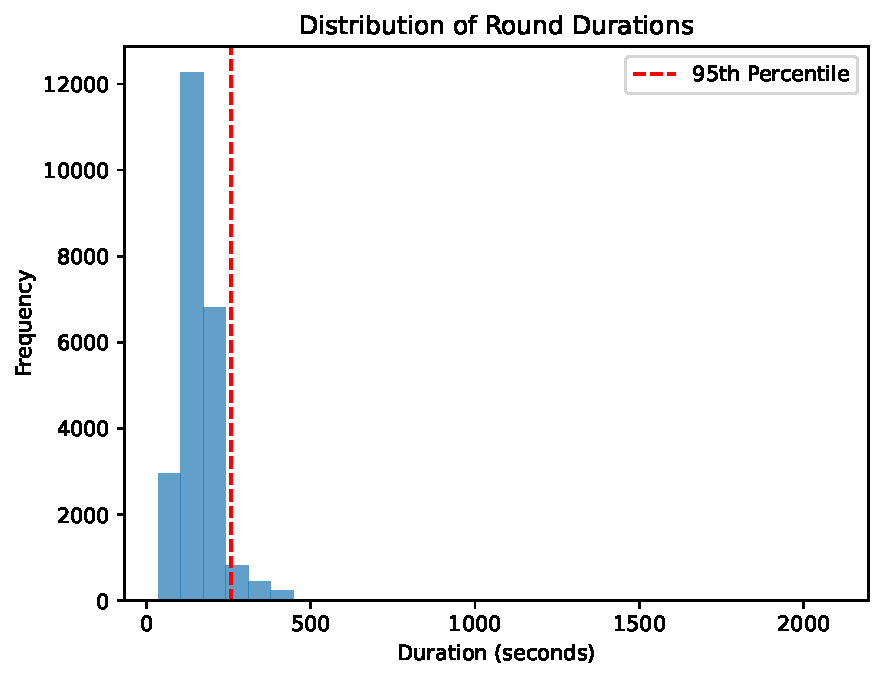
\includegraphics[width=0.9\linewidth]{round_duration_dist.pdf}
  \caption{Distribution of round durations across 464 CS2 matches. A red dashed line marks the 95th percentile, which is used to cap this feature during normalization.}
  \label{fig:round_duration_dist}
\end{figure}

\smallskip

The score is used as a feature for our input vector. This is normalized as such:

\begin{equation}
  \text{Score}_{T, norm} = \frac{\text{Score}_{T}}{\text{Max Rounds Possible}}, \quad T \in \{\text{A}, \text{B}\}
\end{equation}

\medskip

However, round number proved to be another feature that needed appropriate bound handling. In \textit{CS2} rounds can exceed past the twelve round if teams tie, leading into overtime. In theory, \textit{CS2} matches could have infinite rounds. In order to appropriately scale round numbers, we observed the 95th percentile across all accumulated match data.

\smallskip

\begin{figure}[ht]
  \centering
  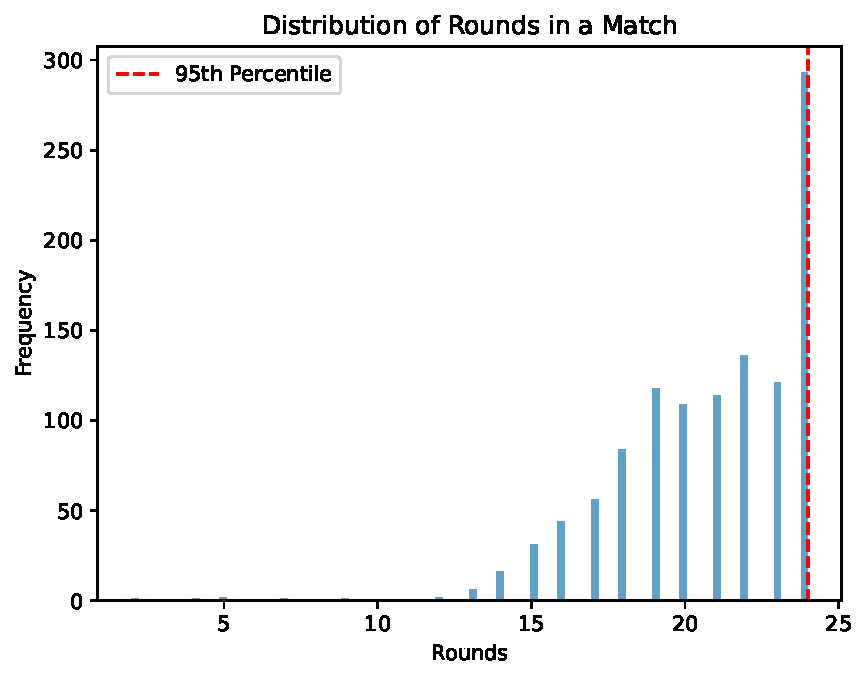
\includegraphics[width=0.9\linewidth]{total_rounds_distribution.pdf}
  \caption{Distribution of total rounds of a match across 464 CS2 matches. A red dashed line marks the 95th percentile, which is used to cap this feature during normalization.}
  \label{fig:round_duration_dist}
\end{figure}

\smallskip

Our dataset does not include overtime rounds, which are common in closely contested matches that exceed the standard 24-round regulation period. This introduces a potential limitation in training stability, as the agent may develop an implicit bias against matches with extended durations or fail to learn strategies that are relevant in overtime contexts.

While acknowledging this gap, we chose to exclude overtime rounds due to time constraints and the added complexity of scraping and preprocessing additional match data. Incorporating overtime rounds remains a promising direction for future work, as doing so would allow for more robust agent generalization and greater realism in match simulation.

We also examined the distribution of a team's round level ROI. To visualize the spread across teams, we used a violin plot to highlight both the density and variance in ROI outcomes.

\begin{figure}[ht]
  \centering
  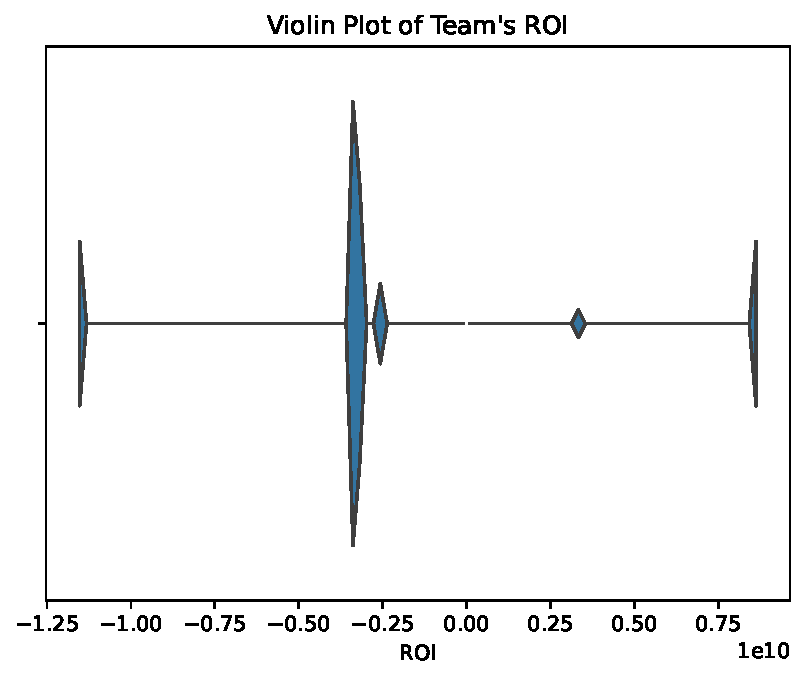
\includegraphics[width=0.9\linewidth]{roi_violin.pdf}
  \caption{Distribution of a team's ROI based on their economic performance.}
  \label{fig:round_duration_dist}
\end{figure}

\smallskip

As seen in Figure 3, the distribution is highly skewed, with a small number of rounds producing extreme positive or negative values. To stabilize this feature for training, we cap ROI at the 99th percentile with an absolute value of 24.0 and apply a signed log transformation. This preserves information while compressing extreme magnitudes, improving stability and preventing outlier dominance during learning.

Lasty, in order to encode the match outcome, we apply one-hot encoding to the winner label, resulting in a two-dimensional binary vector indicating whether Team A or Team B won \cite{datacamp_onehot_2023}. This representation avoids introducing ordinal bias into the model and ensures compatibility with neural network inputs."

\begin{align*}
\text{Team A win} &\rightarrow [1,\ 0] \\
\text{Team B win} &\rightarrow [0,\ 1]
\end{align*}


\subsection{Control Variable}

In order to verify that rich market signals provided an advantage, we employed an \textit{Agent 0} as our ground level experiment. This agent would not use any sophisticated signals and rely on the raw game state features from scraping. \textit{Agent 0} includes the variables previously defined as such:

\begin{equation}
  \text{Score}_{T},
  \text{Kills}_{T},
  \text{Duration}_{round}
\end{equation}

Additionally, since the agent does not utilize advanced economic signals such as delta economy, expected value (EV), or the Kelly Criterion, we introduce a categorical feature known as the \textit{buy type}. During the buy phase, each team allocates funds that can be categorized into one of four discrete tiers based on spending hierarchy: \textit{eco}, \textit{force}, \textit{semi-buy}, and \textit{full-buy}. These categories offer a simplified yet informative heuristic derived directly from game state data, without requiring external calculations.

For each team \( T \in \{\text{A}, \text{B}\} \), buy types are one-hot encoded as follows:

\begin{align}
\text{Buy Type}_T(\text{eco})      &= [1,\ 0,\ 0,\ 0,\ 0] \nonumber \\
\text{Buy Type}_T(\text{force})    &= [0,\ 1,\ 0,\ 0,\ 0] \nonumber \\
\text{Buy Type}_T(\text{semi-buy}) &= [0,\ 0,\ 1,\ 0,\ 0] \nonumber \\
\text{Buy Type}_T(\text{full-buy}) &= [0,\ 0,\ 0,\ 1,\ 0] \nonumber \\
\text{Buy Type}_T(\text{unknown})  &= [0,\ 0,\ 0,\ 0,\ 1]
\end{align}

We include an additional \textit{unknown} flag to account for instances where a team’s buy type cannot be reliably determined. This preserves contextual integrity without introducing artificial bias into the model input.

\section{PPO Model Overview}

PPO is a policy gradient reinforcement learning algorithm. PPO is inteneded to optimize the policy performance while maintaining training stability. This algorithm was developed by researchers at Open AI, introduced in 2017 by Schulman et al \cite{schulman2017proximalpolicyoptimizationalgorithms}. This was a simpler alternative to Trust Region Policy Optimization (TRPO).

Unlike TRPO, which relied on complex second-order optimization, PPO uses a clipped surrogate objective that restricts policy updates to stay within a safe range. The clipping mechanism helps stabilize learning by preventing excessive policy shifts, which risk training stability. PPO is favored for its ease of implementation and sample efficiency. PPO is also noted for strong empirical performance across continuous and discrete action space \cite{schulman2017proximalpolicyoptimizationalgorithms}.

Our project employs PPO to train a betting agent that makes decisions based on game features described above. While using strong market financial signals, we aimed to evaluate perfomance comparing against agents using various reward and action spaces.

\subsection{Model Choice}

   For our PPO structure, we used a popular model found on \textit{GitHub} developed by Nikhil Barhate \cite{barhate2020ppo}. In their implementation, the actor-critic use a shared network structure. Initial layers of the unified neural network process input states and then split into two separate heads: one for the actor and another for the critic. This allows for both the policy and value function to share common layers, reducing redundancy and computation overhead.

   To guide policy and value function updates, the advantage function is estimated using Monte Carlor returns. For each time step in an episode, the agent computes the cumulative discounted reward based on the full trajectory. This serves as an estimate for how favorable a given state-action pair was compared to the baseline value function. While this method introduces higher variance compared to bootstrapped alternatives like Generalized Advantage Estimation (GAE), this advantage estimation provides a straightforward way to compute advantages from complete episode data. 

\subsection{Hyperparameters}

We selected these hyperparameters based on values recommended in the original PPO paper \cite{schulman2017proximalpolicyoptimizationalgorithms}, which have been shown to work well across a range of tasks. They offer a strong baseline for stable training without extensive tuning, allowing us to focus on adapting PPO to the betting domain.

\begin{table}[h]
  \caption{PPO Hyperparameters}
  \label{tab:ppo-hyperparams}
  \begin{tabular}{@{}ll@{}}
    \toprule
    \textbf{Hyperparameter} & \textbf{Value} \\
    \midrule
    Actor learning rate & 0.0003 \\
    Critic learning rate & 0.001 \\
    Discount factor ($\gamma$) & 0.99 \\
    Epochs per update ($K_{\text{epochs}}$) & 80 \\
    Clipping parameter ($\epsilon_{\text{clip}}$) & 0.2 \\
    Continuous action space & \texttt{false (except for Agent 4)} \\
    Initial action std.\ dev.\ & 0.6 \\
    Device & \texttt{device} \\
    \bottomrule
  \end{tabular}
\end{table}

Our hyper parameters are shown in Table 1. Agent 4 is an additional thought experiment to validate whether or not a non-discrete action space results to poor performance.

\section{Training Procedure}

Our project aims to evaluate multiple agent configurations by varying reward functions and action spaces. The choice of reward function plays a critical role in shaping agent behavior, as poorly designed rewards can hinder effective learning.

While betting naturally lends itself to a continuous action space, allowing for flexible wager sizes, we constrain the action space to a discrete set of options for training simplicity and stability.

During both training and testing, the agent could place or change a bet at the start of every round, using updated game state information before each decision. In reality, once you place a wager on a sportsbook, it is locked in for the entire match and cannot be adjusted mid‐game; our simulation instead lets the agent freely revise its bet each round to learn from finer grained outcomes. This approach sacrifices realism, since real bets cannot be changed. This overestimate performance, but it was chosen to simplify implementation and fit our time scope.

\subsection{Feature Choice}

We trained two versions of our PPO agent using different feature representations. The raw feature vector consists of unprocessed game state information (as previously described for Agent 0), directly reflecting the state of play. In contrast, the crafted feature vector includes additional market-derived signals such as odds, ROI, and betting indicators. This allows the agent to learn not just from gameplay data, but also from financial cues that influence real-world betting decisions.

Agents using a complex reward function must be assigned a bankroll, since the reward is based on the percentage of their stake. Unlike binary win or loss signals, this setup models profit or loss relative to how much the agent bets, making bankroll management an essential part of the learning process.

\begin{table}[h]
  \caption{Agent Comparison Across Feature Vector Choice}
  \label{tab:agent_benchmarks}
  \begin{tabular}{lccccc}
    \toprule
    \textbf{Agent} & \textbf{Raw Feature} & \textbf{Crafted Feature} \\
    \midrule
    Agent 0 (no bankroll/signals)     & \cmark  &        \\
    Agent 1 (no bankroll)     & \cmark  &        \\
    Agent 2 (w/ bankroll)   &         & \cmark \\
    Agent 3 (w/ bankroll)   &         & \cmark \\
    \bottomrule
  \end{tabular}
\end{table}

\subsection{Reward Function Exploration}

Reward function is calculated as:
\[
r: (\text{action},\ \text{outcome}) \rightarrow \mathbb{R}
\]

Our basic binary reward function is defined as:

\begin{equation}
r_{\text{binary}} =
\begin{cases}
+1, & \text{if bet is correct} \\
-1, & \text{if bet is incorrect} \\
\phantom{+}0, & \text{if no bet is placed}
\end{cases}
\end{equation}

Our complex discrete reward function is defined as:

\begin{equation}
r_{\text{discrete}} =
\begin{cases}
\text{Stake} \times (\text{Odds} - 1), & \text{if bet is correct} \\
-\text{Stake}, & \text{if bet is incorrect} \\
\text{0}, & \text{if no bet is placed}
\end{cases}
\end{equation}

A visual overview of our agent distribution across reward functions is as follows:

\begin{table}[h]
  \caption{Agent Comparison Across Reward Functions}
  \label{tab:agent_benchmarks}
  \begin{tabular}{lccccc}
    \toprule
    \textbf{Agent} & \textbf{Binary} & \textbf{Discrete} \\
    \midrule
    Agent 0 (no bankroll/signals)     & \cmark  &        \\
    Agent 1 (no bankroll)     & \cmark  &        \\
    Agent 2 (w/ bankroll)   &         & \cmark \\
    Agent 3 (w/ bankroll)   &         & \cmark \\
    \bottomrule
  \end{tabular}
\end{table}

\subsection{Action Space Definitions}

A basic action space is defined as a discrete space of three actions: abstaining, betting on team A, or betting on team B.

\begin{equation}
\mathcal{A}_{\text{basic}} = \{\text{abstain}, \text{bet A}, \text{bet B} \}
\end{equation}

A complex discrete action space is defined as a discrete space of nine actions: abstaining, betting $\{5, 10, 25, 50\}$ percent of agent's bankroll on either team A or B

\begin{equation}
\mathcal{A}_{\text{discrete}} = \{\text{abstain}\} \cup \{(t, p) \mid t \in \{\text{A}, \text{B}\},\ p \in \{5\%, 10\%, 25\%, 50\%\} \}
\end{equation}

With two different reward functions and action spaces, our project compares the perfomance of three different agents using various combinations. These three agents are defined as so: 


\begin{table}[h]
  \caption{Agent Comparison Across Action Spaces}
  \label{tab:agent_benchmarks}
  \begin{tabular}{lccccc}
    \toprule
    \textbf{Agent} & \textbf{Basic} & \textbf{Discrete} \\
    \midrule
    Agent 0 (no bankroll/signals)     & \cmark  &         \\
    Agent 1 (no bankroll)               & \cmark  &         \\
    Agent 2 (with bankroll)             & \cmark  &         \\
    Agent 3 (with bankroll)             &         & \cmark  \\
    \bottomrule
  \end{tabular}
\end{table}

\subsection{Agent 4}

We also benchmarked an agent that used a complex reward function and used a continuous action space. This was to demonstrate and experiment how a large non-discrete action space would performe against discrete actions.

\begin{table}[h]
  \caption{Agent Comparison Across Reward Functions}
  \label{tab:agent_benchmarks}
  \begin{tabular}{lccccc}
    \toprule
    \textbf{Agent} & \textbf{Complex R.} & \textbf{Continuous A.} & \textbf{Crafted} \\
    \midrule
    Agent 4 (w/ bankroll)   & \cmark        & \cmark & \cmark\\
    \bottomrule
  \end{tabular}
\end{table}

\bigskip
\section{Experiments and Results}

To evaluate the training progress and behavior of our reinforcement learning agent, we log and visualize several key metrics throughout the training process. Figure~\ref{fig:training_metrics} summarizes these insights.

\bigskip

The \textbf{Cumulative Reward} graph illustrates the total reward accumulated by the agent over time, providing a high-level view of learning progression. 

\begin{figure*}[t]
  \centering
  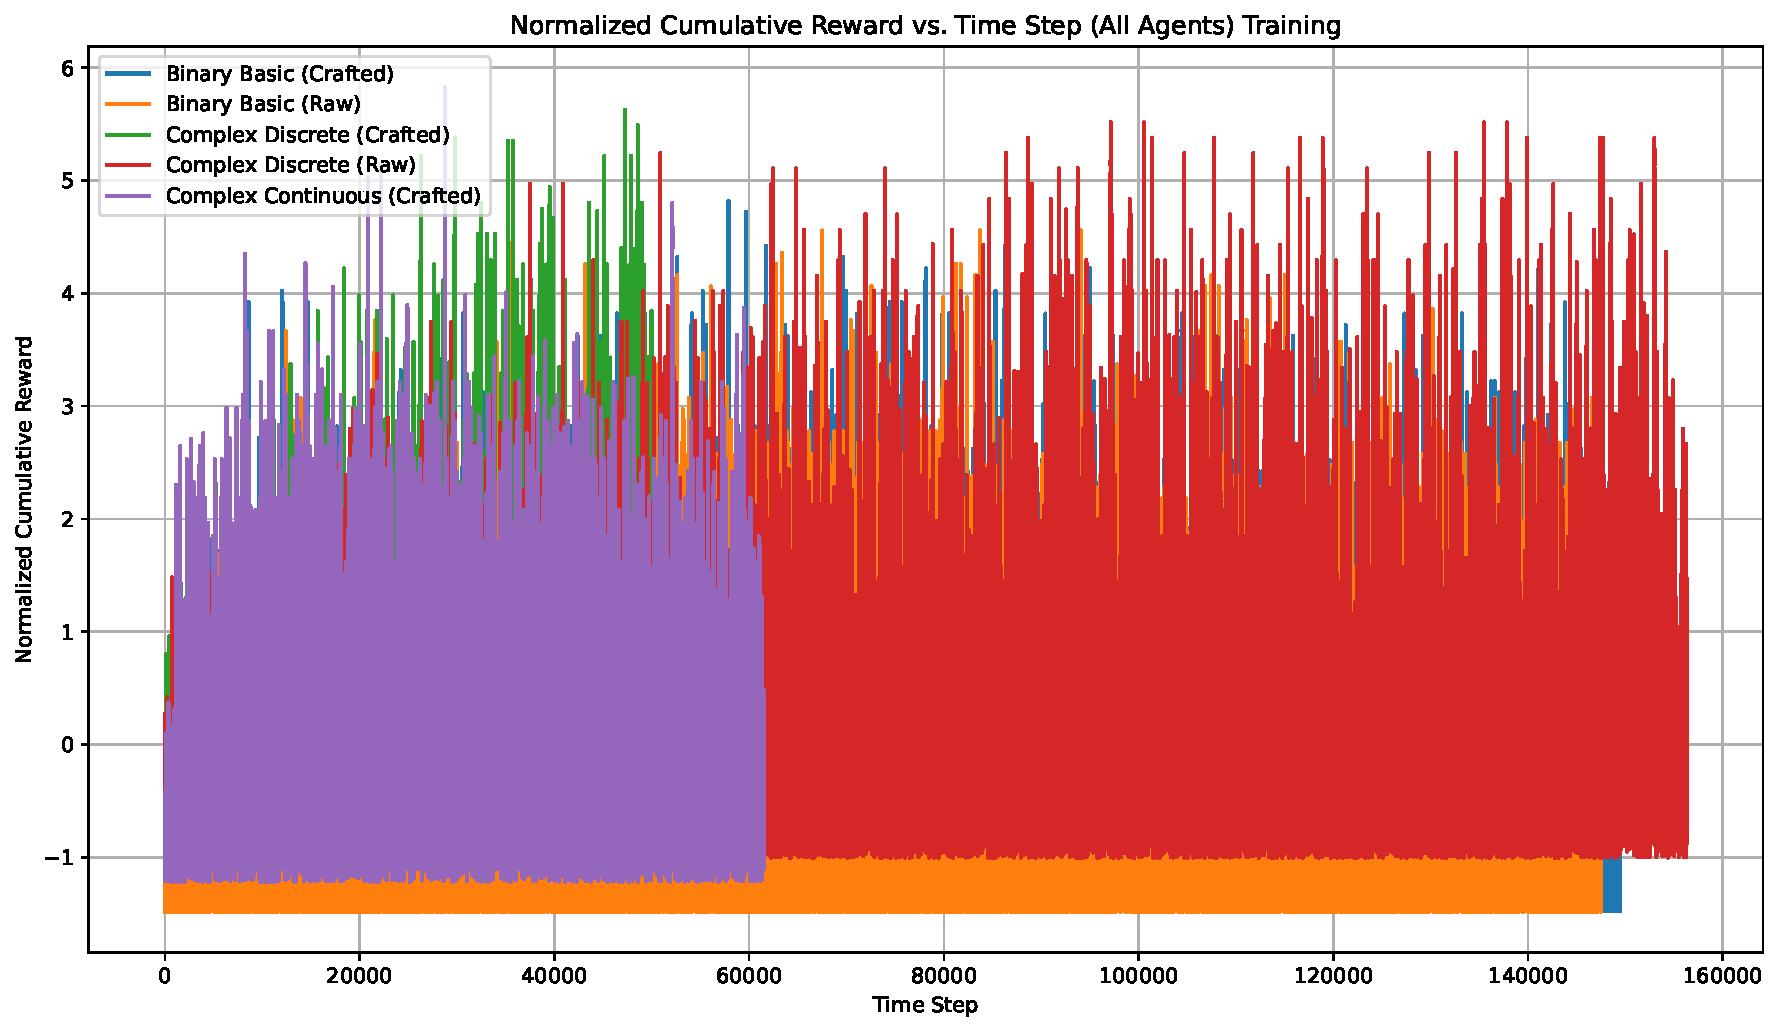
\includegraphics[width=\textwidth]{cumulative_reward_all_training.pdf}
  \caption{Cumulative reward during the training phase (all agents).}
  \label{fig:cumulative_reward_all_training}
\end{figure*}

\bigskip

Early in training (up to roughly 20,000 steps), all agents begin near zero; the \emph{Complex Continuous (Crafted)} agent (purple) rapidly climbs to a normalized reward of about 2 by 30,000 steps and then maintains a relatively stable plateau between 1.5 and 3, indicating that leveraging continuous profit signals alongside rich economic features helps the policy stabilize more quickly. In contrast, the \emph{Binary Basic (Raw)} agent (orange) remains nearly flat (around –1) throughout training, demonstrating that a simple $\pm1$ reward without economic context fails to guide meaningful learning. The \emph{Binary Basic (Crafted)} agent (blue) shows modest improvement over the raw version, reaching normalized rewards near 1 by 100,000 steps, which suggests that even a basic reward can benefit from added economic features. The \emph{Complex Discrete (Raw)} agent (red) exhibits high variance with large positive spikes (up to 5–6) but remains noisy and does not settle, indicating that a complex discrete reward alone can produce occasional large gains but lacks consistency. When the same discrete reward is combined with crafted features (\emph{Complex Discrete (Crafted)}, green), the agent converges faster—reaching around 3 by 40,000 steps—before the training curve ends at 60,000 steps; this early convergence suggests that feature engineering reduces variance and accelerates learning in the discrete‐reward setting. Overall, Figure~\ref{fig:cumulative_reward_all_training} demonstrates that richer reward formulations and the inclusion of economic and market‐derived features both improve convergence speed and lead to higher, more stable cumulative rewards compared to raw or binary reward functions alone.

\bigskip

\begin{figure*}[t]
  \centering
  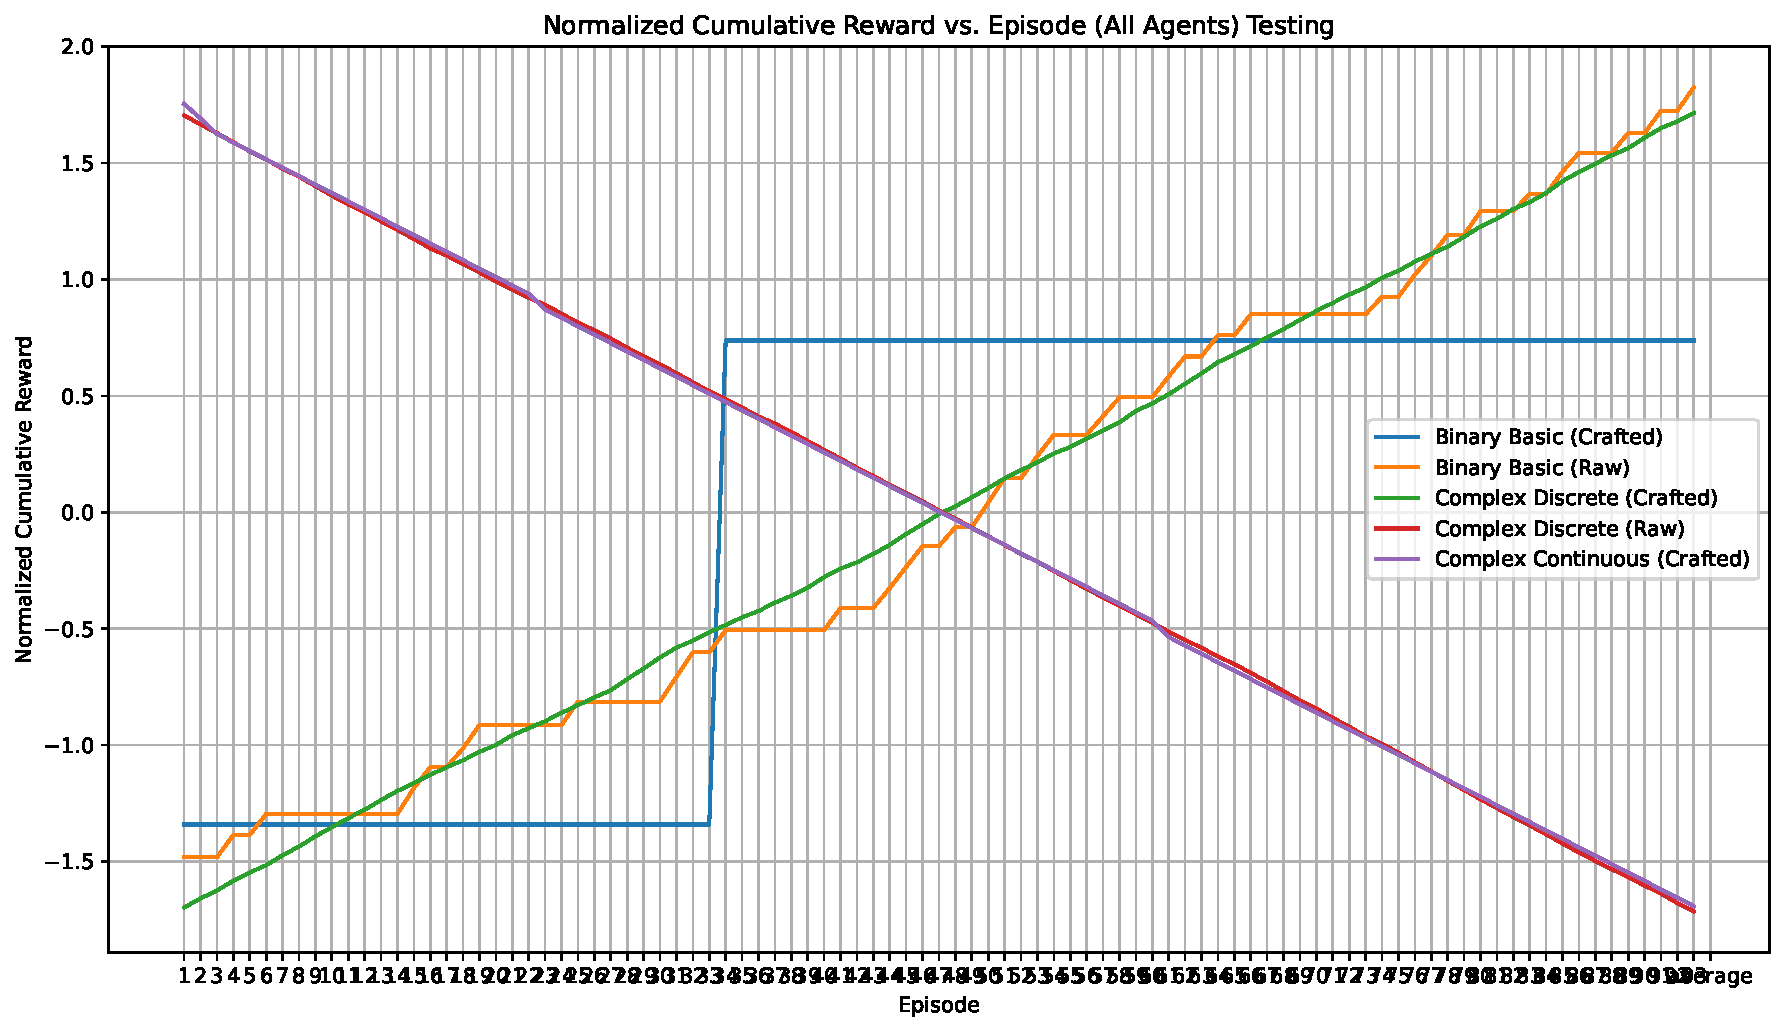
\includegraphics[width=\textwidth]{cumulative_reward_all_testing.pdf}
  \caption{Cumulative reward during the training phase (all agents).}
  \label{fig:cumulative_reward_all_testing}
\end{figure*}

The \textbf{Policy and Value Loss} graph tracks the agent's optimization process, where decreasing policy loss indicates stabilization in policy updates, and decreasing value loss reflects improved estimation of expected returns. 

\bigskip

Across all five agents, incorporating crafted features consistently leads to lower and more stable policy and value losses compared to raw‐feature counterparts. In the binary reward setting, the Binary Basic (Raw) agent exhibits persistently high and noisy losses, whereas Binary Basic (Crafted) shows a gradual downward trend and reduced variance. For the Complex Discrete agents, the (Crafted) version converges most quickly—policy and value losses fall near zero by around episode 2000—while the raw variant remains erratic and slower to decrease. The Complex Continuous (Crafted) agent begins with higher initial loss but steadily declines thereafter, in contrast to its raw counterpart, which oscillates more throughout training. Overall, feature engineering not only accelerates convergence—especially for discrete rewards—but also dampens loss spikes, producing smoother learning curves.

\bigskip

\begin{figure*}[t]
  \centering
  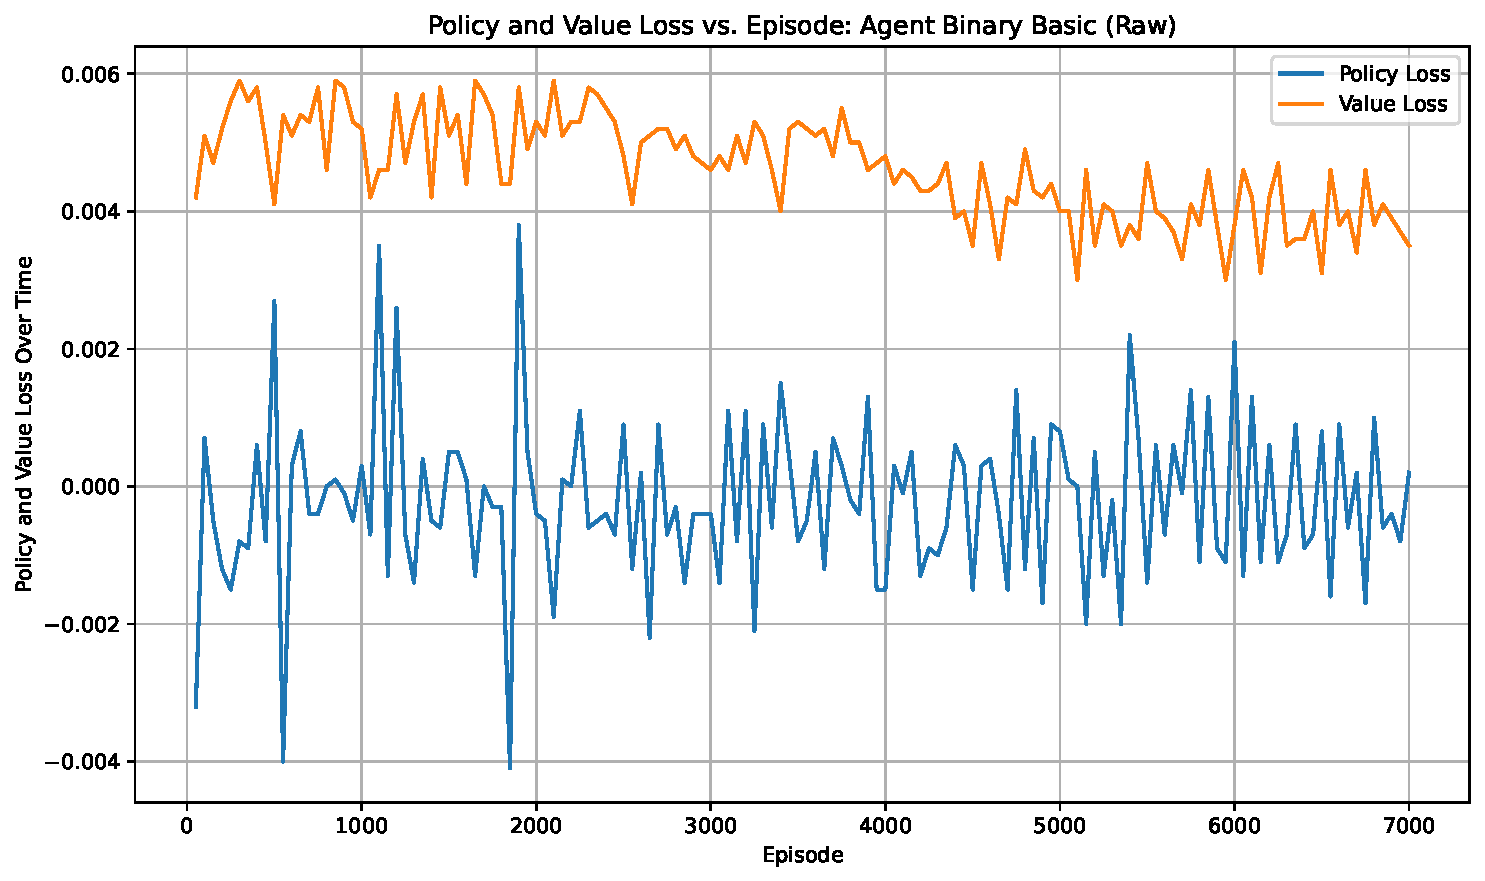
\includegraphics[width=\textwidth]{policy_value_loss_Binary Basic (Raw).pdf}
  \caption{Cumulative reward during the training phase (all agents).}
  \label{fig:policy_value_loss_Binary Basic (Raw)}
\end{figure*}

\begin{figure*}[t]
  \centering
  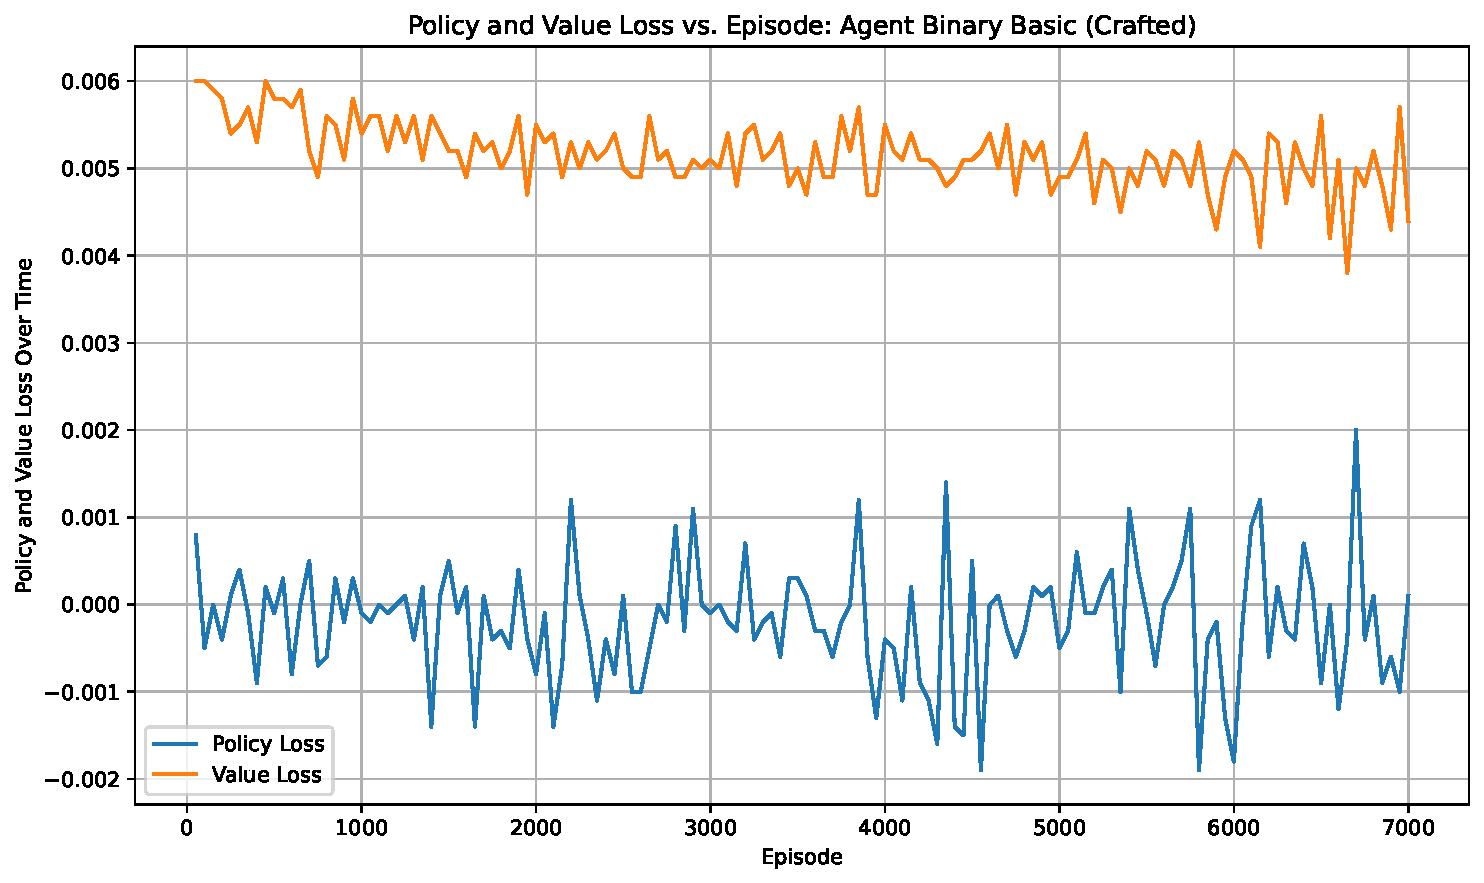
\includegraphics[width=\textwidth]{policy_value_loss_Binary Basic (Crafted).pdf}
  \caption{Cumulative reward during the training phase (all agents).}
  \label{fig:policy_value_loss_Binary Basic (Crafted)}
\end{figure*}


\begin{figure*}[t]
  \centering
  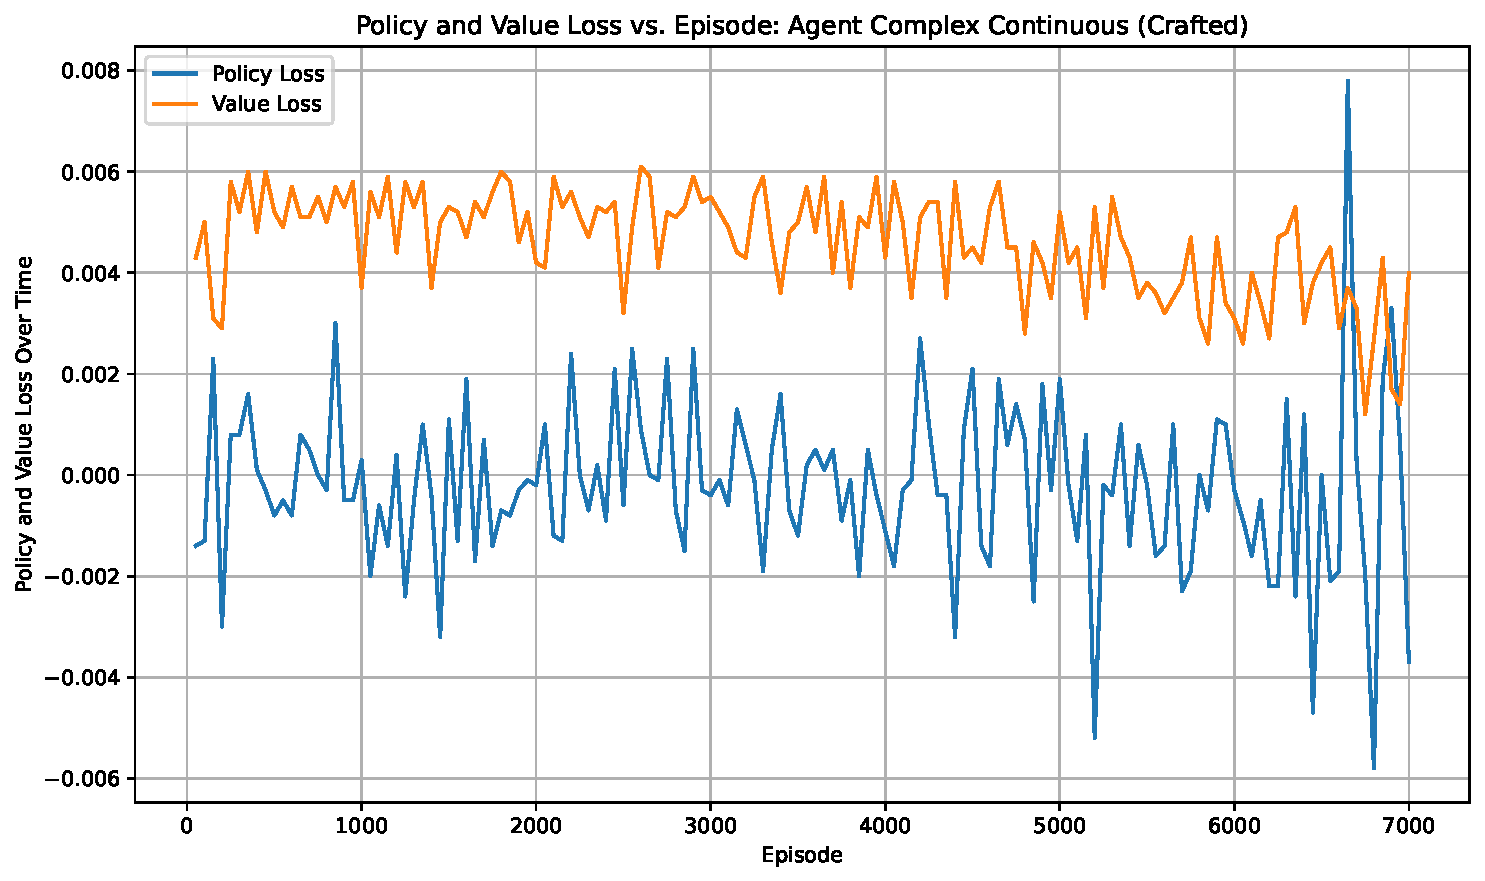
\includegraphics[width=\textwidth]{policy_value_loss_Complex Continuous (Crafted).pdf}
  \caption{Cumulative reward during the training phase (all agents).}
  \label{fig:policy_value_loss_Complex Continuous (Crafted)}
\end{figure*}


\begin{figure*}[t]
  \centering
  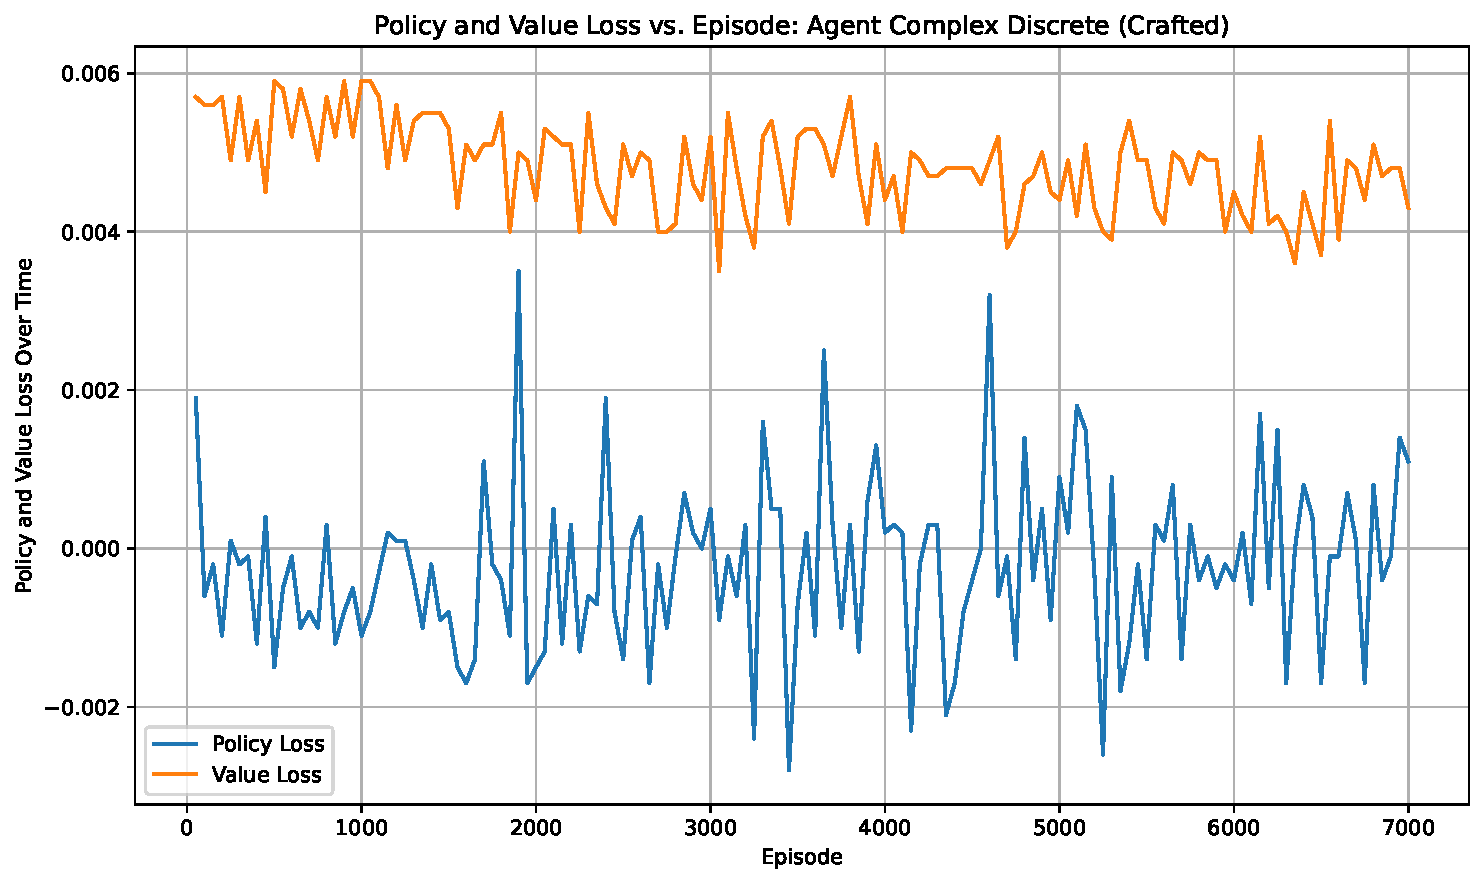
\includegraphics[width=\textwidth]{policy_value_loss_Complex Discrete (Crafted).pdf}
  \caption{Cumulative reward during the training phase (all agents).}
  \label{fig:policy_value_loss_Complex Discrete (Crafted)}
\end{figure*}

\begin{figure*}[t]
  \centering
  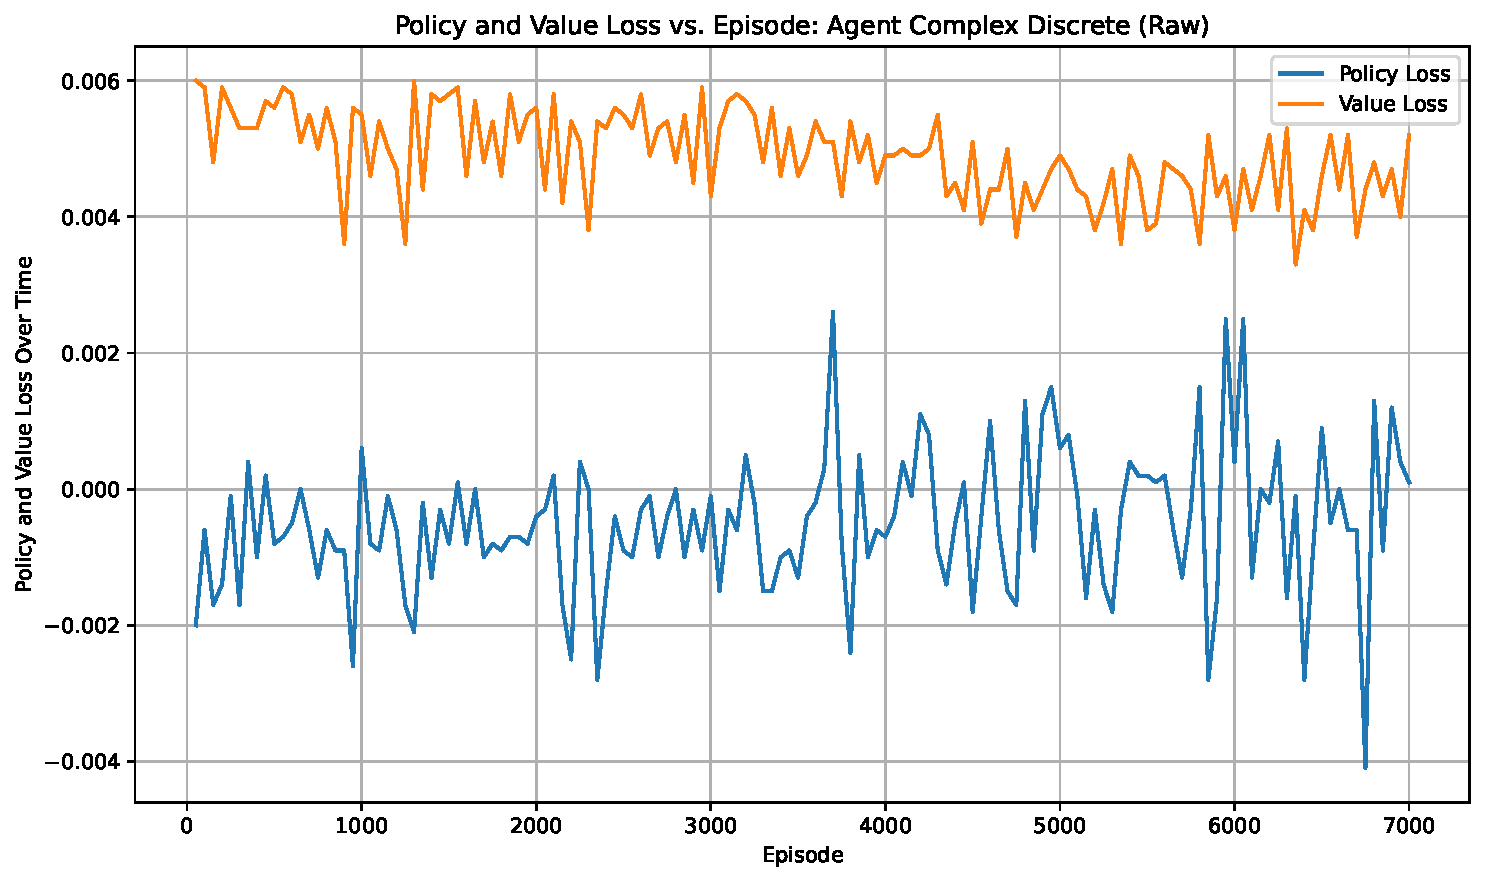
\includegraphics[width=\textwidth]{policy_value_loss_Complex Discrete (Raw).pdf}
  \caption{Cumulative reward during the training phase (all agents).}
  \label{fig:policy_value_loss_Complex Discrete (Raw)}
\end{figure*}

The \textbf{Return Distribution} graph visualizes the spread of cumulative episode rewards; a tighter cluster around higher values suggests improved and consistent performance.

\bigskip

The return‐distribution histograms show that agents with crafted features have much tighter, higher‐centered reward clusters, whereas raw‐feature agents display wide, low‐centered spreads. For example, the \emph{Binary Basic (Crafted)} agent’s returns concentrate around modest positive values (mostly 0–60), while \emph{Binary Basic (Raw)} has a scattered spread up to ~600 with many near‐zero outcomes . In the discrete‐reward setting, \emph{Complex Discrete (Crafted)} returns cluster densely in a high range (0–1.2×10⁶), whereas \emph{Complex Discrete (Raw)} shows a more erratic, lower‐frequency spread up to ~1.6×10⁵. Finally, \emph{Complex Continuous (Crafted)} produces a narrow spike below 100,000, indicating stable gains compared to its raw counterpart. Overall, engineered features lead to more consistent, centrally focused returns, while raw features result in extreme variance and lower median performance.

\bigskip

\begin{figure*}[t]
  \centering
  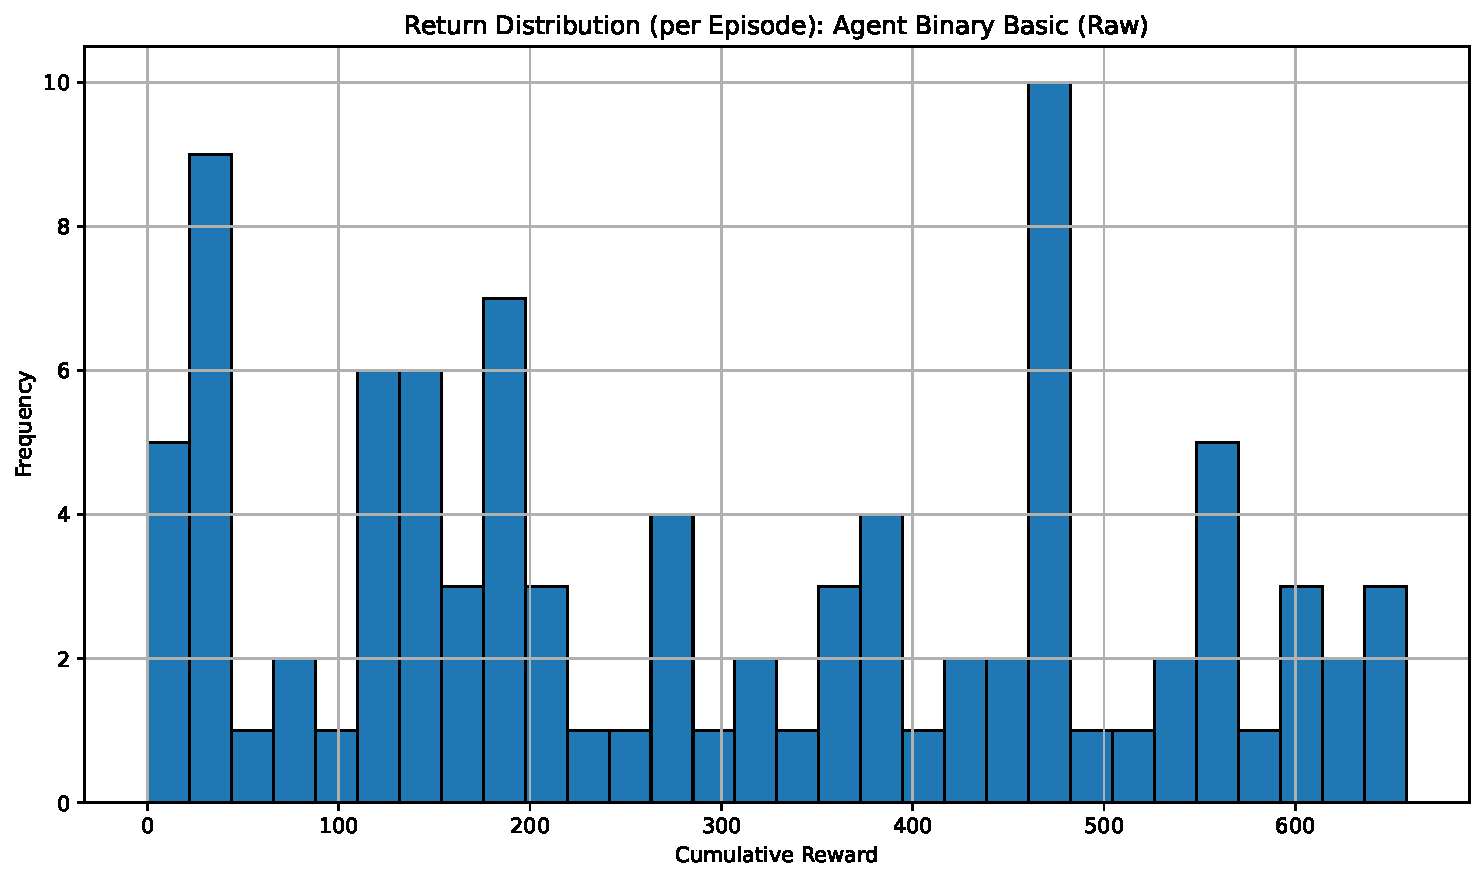
\includegraphics[width=\textwidth]{return_distribution_Binary Basic (Raw).pdf}
  \caption{Cumulative reward during the training phase (all agents).}
  \label{fig:return_distribution_Binary Basic (Raw)}
\end{figure*}

\begin{figure*}[t]
  \centering
  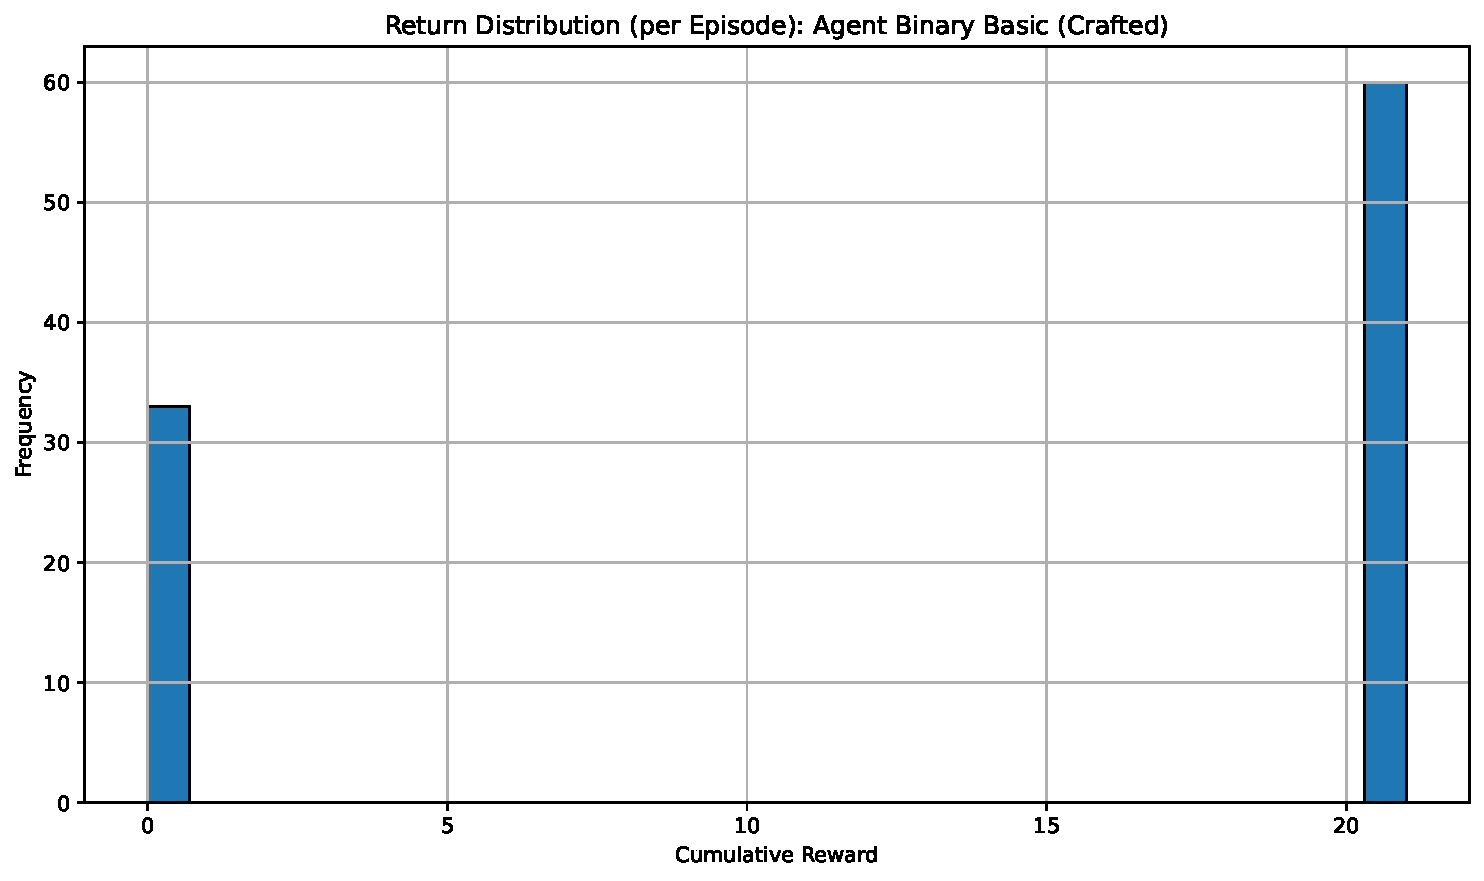
\includegraphics[width=\textwidth]{return_distribution_Binary Basic (Crafted).pdf}
  \caption{Cumulative reward during the training phase (all agents).}
  \label{fig:return_distribution_Binary Basic (Crafted)}
\end{figure*}


\begin{figure*}[t]
  \centering
  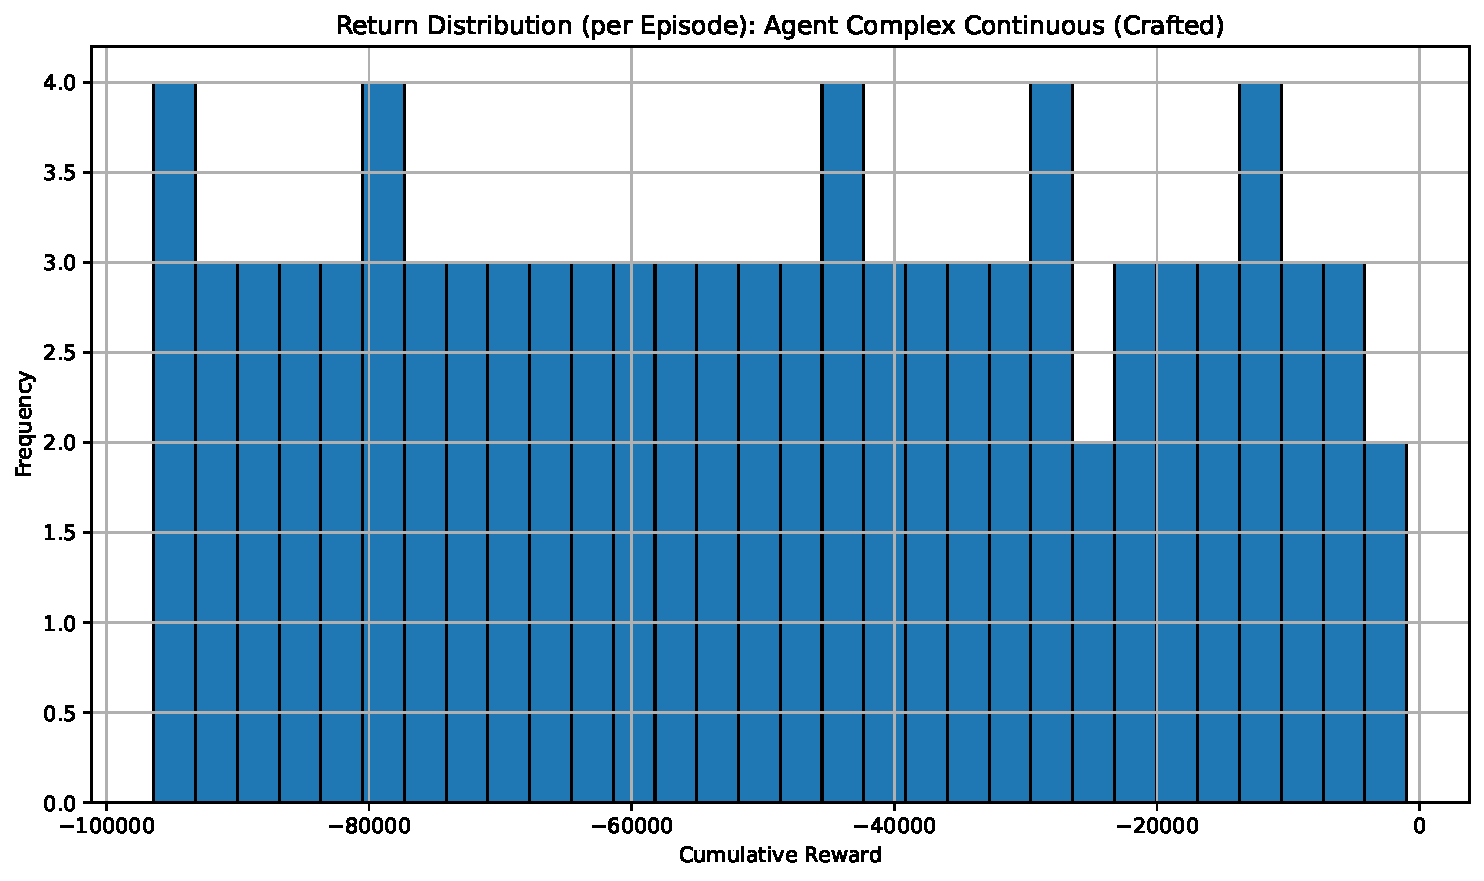
\includegraphics[width=\textwidth]{return_distribution_Complex Continuous (Crafted).pdf}
  \caption{Cumulative reward during the training phase (all agents).}
  \label{fig:return_distribution_Complex Continuous (Crafted)}
\end{figure*}


\begin{figure*}[t]
  \centering
  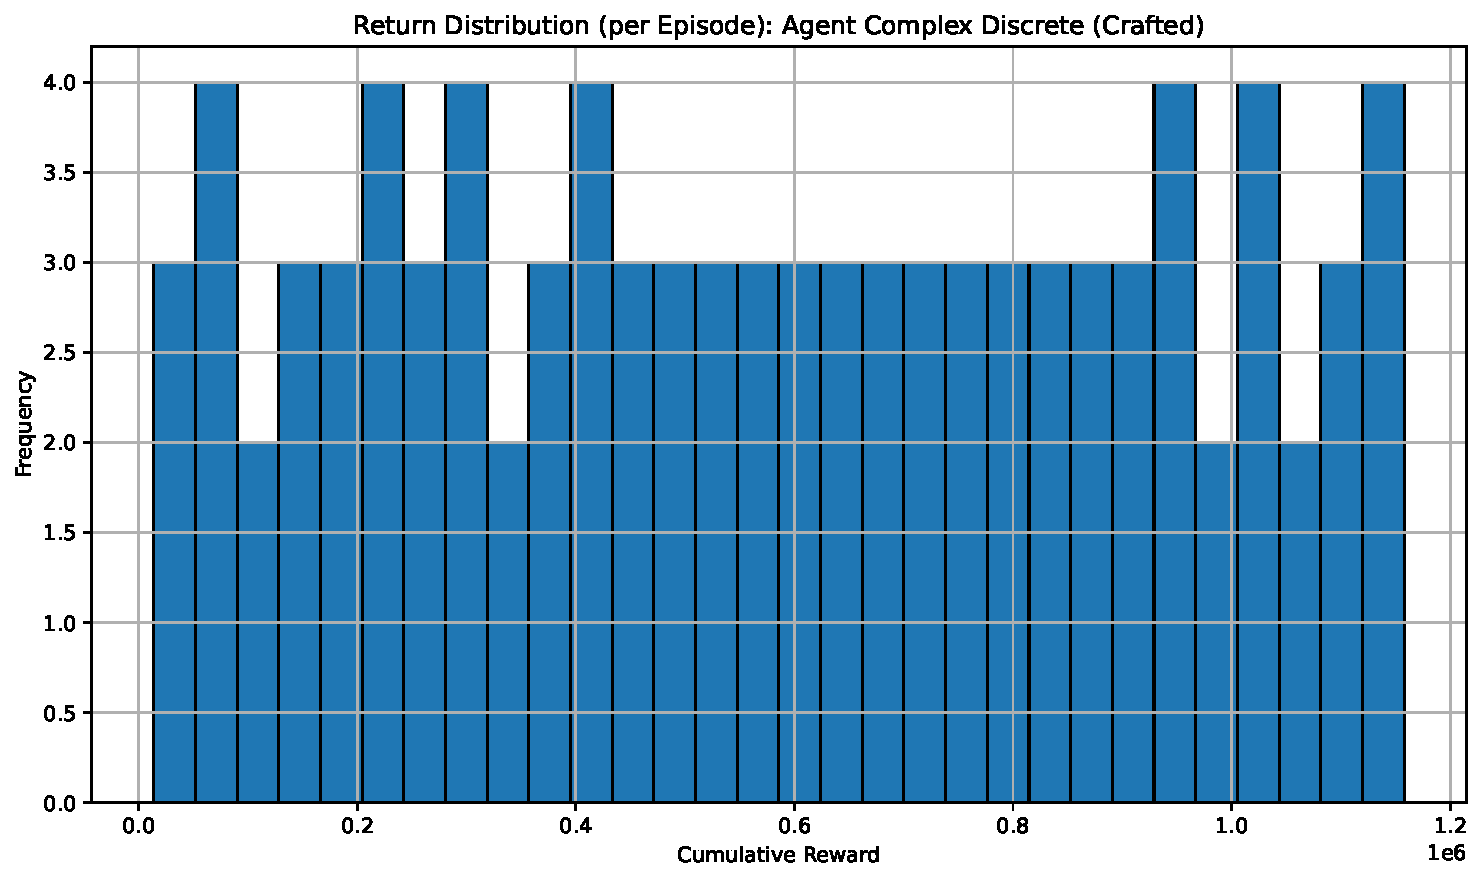
\includegraphics[width=\textwidth]{return_distribution_Complex Discrete (Crafted).pdf}
  \caption{Cumulative reward during the training phase (all agents).}
  \label{fig:return_distribution_Complex Discrete (Crafted)}
\end{figure*}

\begin{figure*}[t]
  \centering
  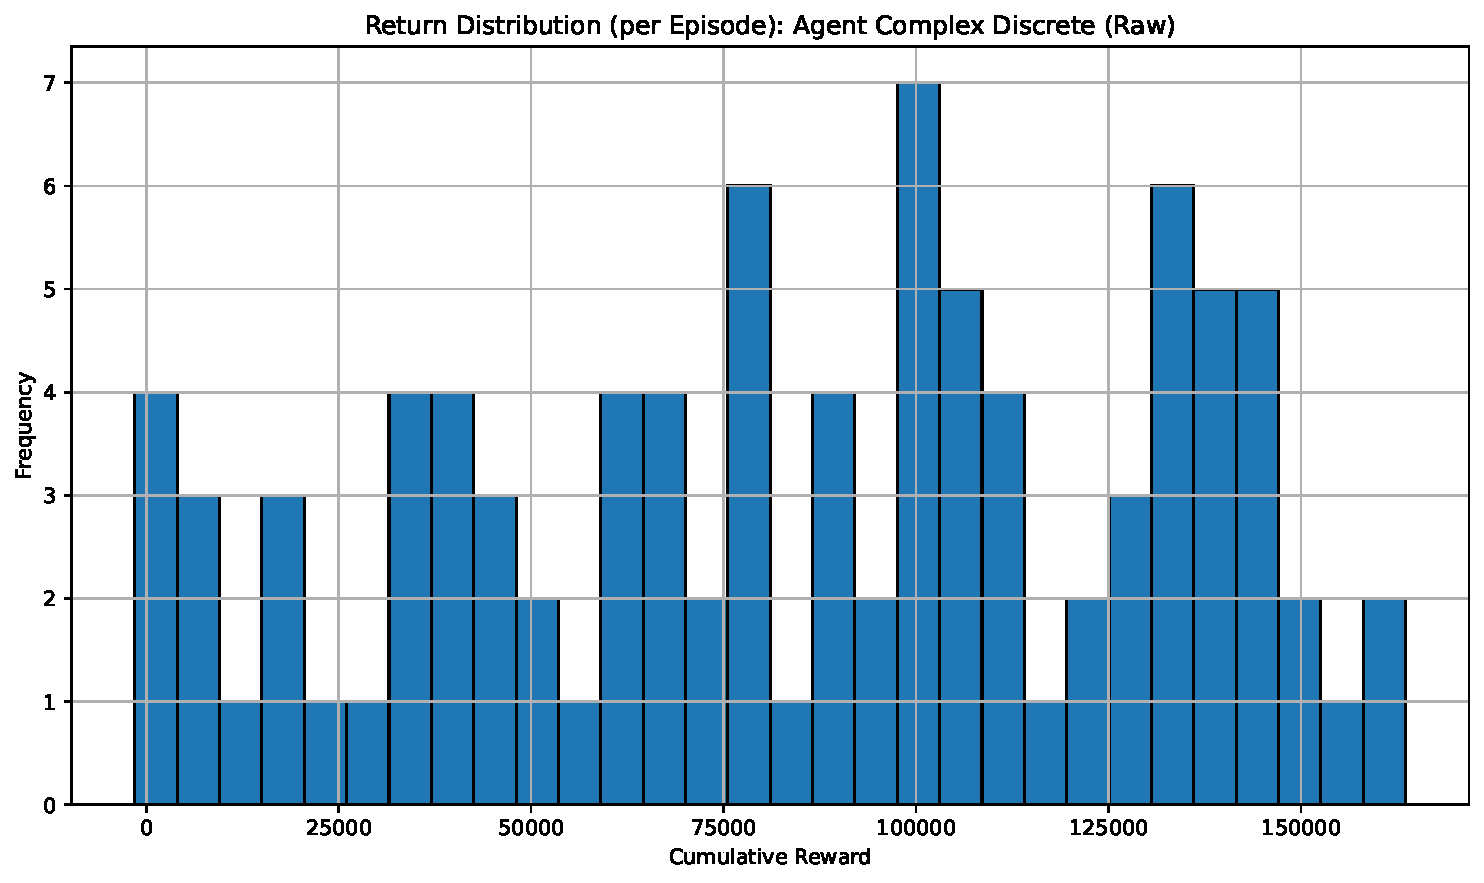
\includegraphics[width=\textwidth]{return_distribution_Complex Discrete (Raw).pdf}
  \caption{Cumulative reward during the training phase (all agents).}
  \label{fig:return_distribution_Complex Discrete (Raw)}
\end{figure*}

The \textbf{Bankroll} graph models the agent's financial trajectory over time, analogous to profit/loss curves in real-world trading or betting scenarios. A sustained upward trend indicates successful policy learning. 

\bigskip

Agents using crafted features exhibit steadier and higher bankroll growth than the raw‐feature agent in both training and testing. During training, the \emph{Complex Discrete (Crafted)} agent’s bankroll climbs smoothly to around \$60{,}000 by 60{,}000 time steps, while the \emph{Complex Discrete (Raw)} agent fluctuates more and stays lower. The \emph{Complex Continuous (Crafted)} agent also outperforms the raw version but lags slightly behind the discrete crafted agent. In testing, the discrete crafted agent again ends with the highest balance, followed by the continuous crafted agent, and the raw agent remains volatile with the lowest final bankroll.

\bigskip

\begin{figure*}[t]
  \centering
  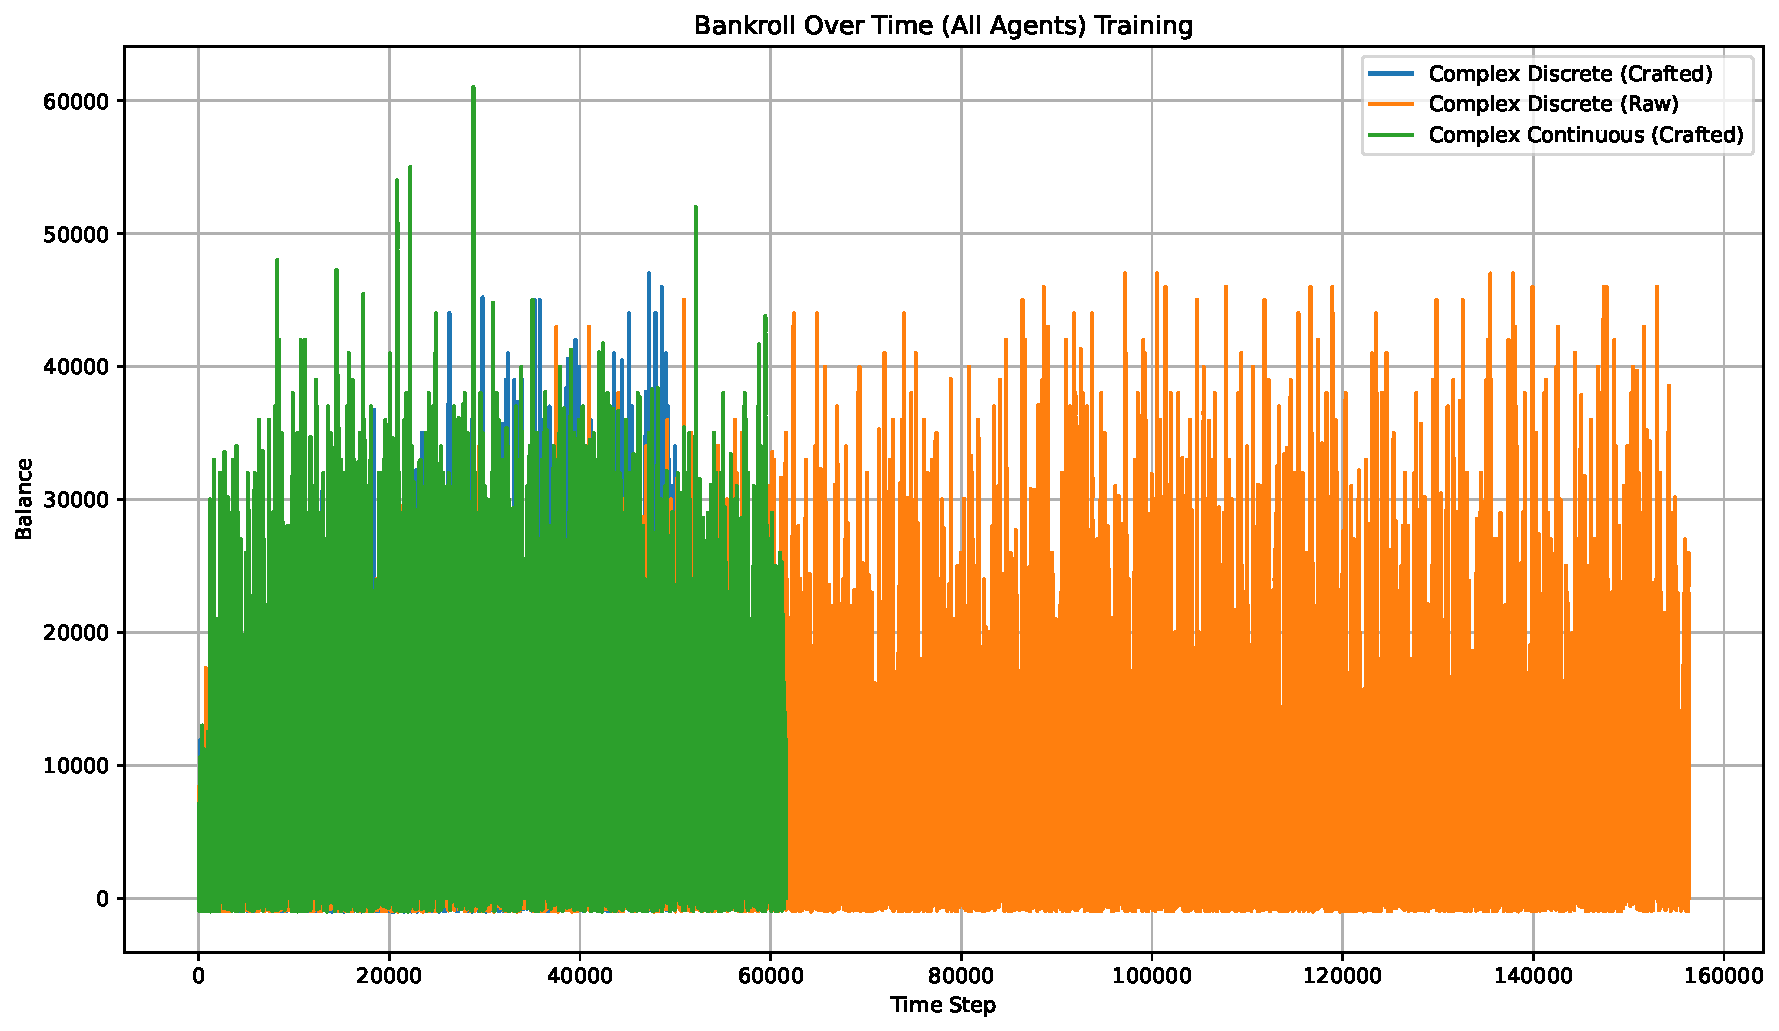
\includegraphics[width=\textwidth]{bankroll_all_training.pdf}
  \caption{Cumulative reward during the training phase (all agents).}
  \label{fig:bankroll_all_training}
\end{figure*}

\begin{figure*}[t]
  \centering
  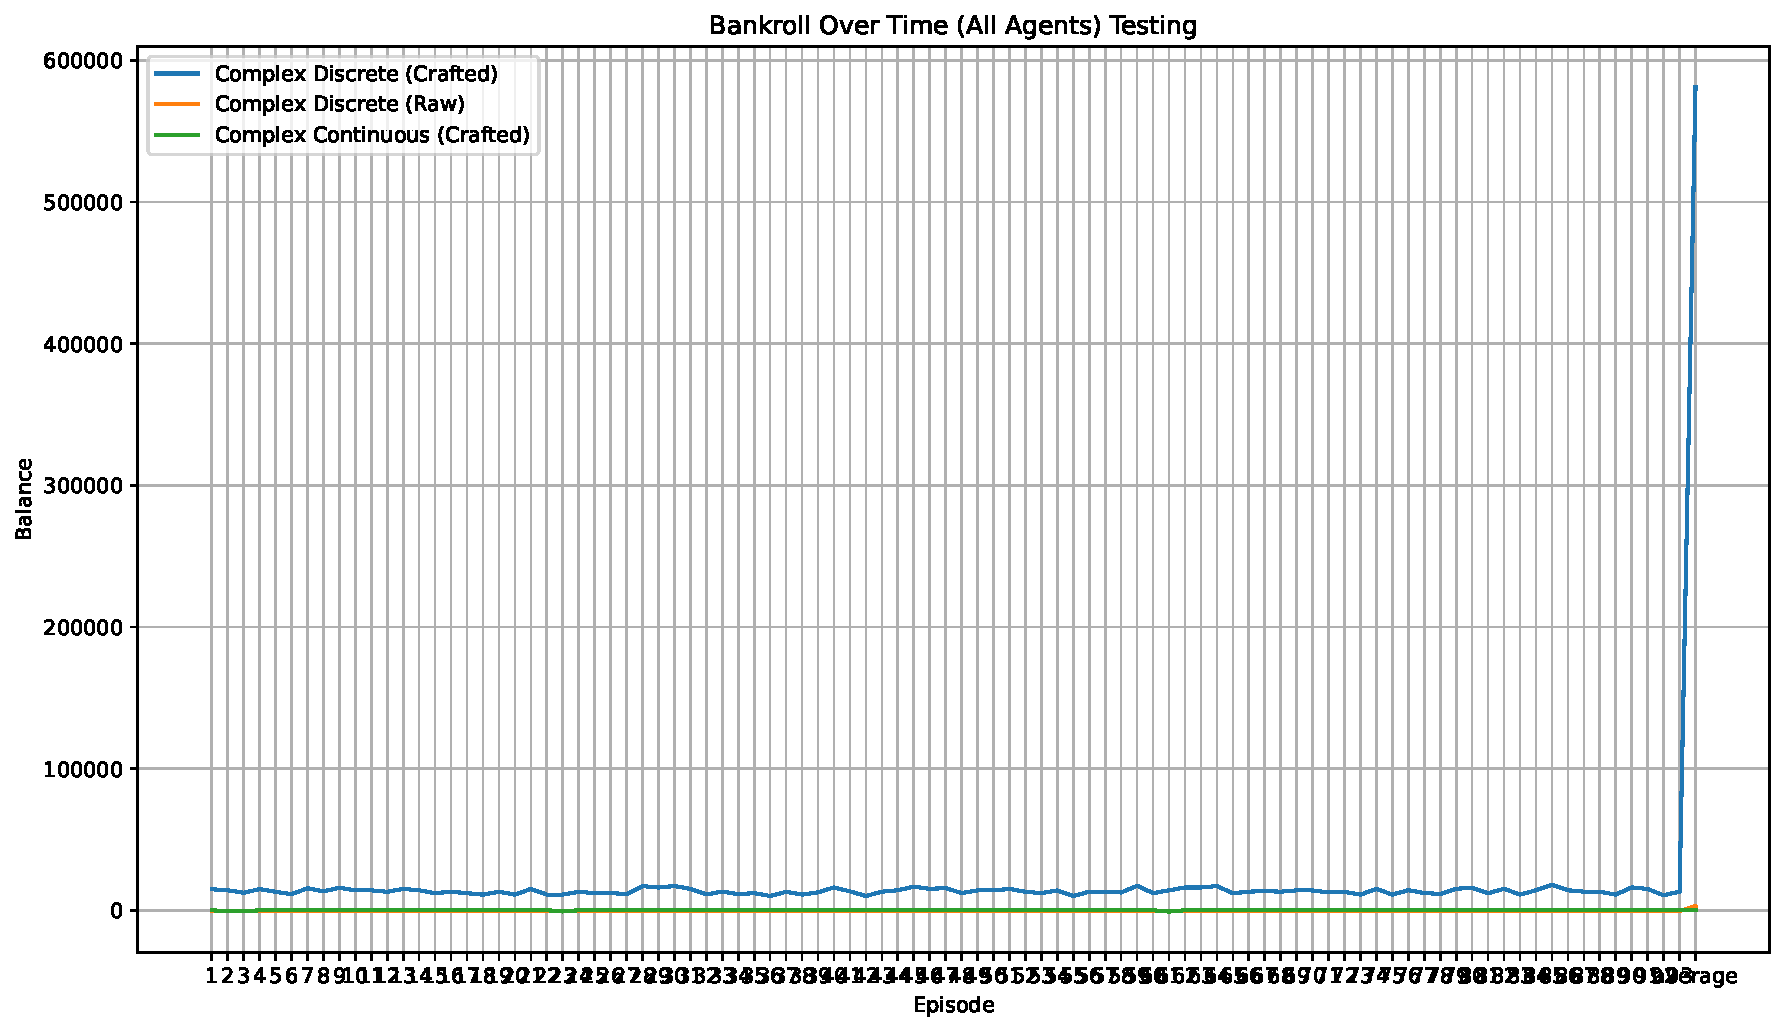
\includegraphics[width=\textwidth]{bankroll_all_testing.pdf}
  \caption{Cumulative reward during the training phase (all agents).}
  \label{fig:bankroll_all_testing}
\end{figure*}

Finally, the \textbf{Probability Calibration} graph compares the agent's predicted win probabilities against actual outcomes. Deviations from the diagonal reflect confidence misalignment—where curves above the diagonal indicate underconfidence, and below indicate overconfidence.

\begin{figure}[ht]
  \centering
  % \includegraphics[width=\linewidth]{training_metrics_placeholder.pdf}
  \caption{Key training metrics tracked during agent development.}
  \label{fig:training_metrics}
\end{figure}


\section{Discussion}

\subsection{Interpretation of Experimental Results}

Our interpretation is.

\subsection{Limitations of PPO in Betting Scenarios}

While PPO has proven effective in continuous control tasks, its application to sports betting context presents several challenges. Firstly, PPO assumes a relatively stable reward structure and a Markovian environment \cite{schulman2017ppo}. However, betting markets, especially in esports, are inherently non-stationary. Odds inevitably flunctuate rapidly based on real-time information. This can happen for various reasons, such as roster changes, game patch updates, and meta shifts. Consequently, the agent's policy is subject to deprecation between training iterations in a long term scope. Thus, without proper updates to the data and tweaks, we can expect suboptimal wagering decisions. Second, PPO's on policy nature requires fresh interaction with data for each update, which can be costly in real-money betting environments.

Gathering sufficiently diverse episodes without incurring large financial risk is difficult. Synthetic or simulated data may lack accurate reflection of live market dynamics \cite{jansen2020rlbetting}. PPO's gradient based update rules can struggle with extremely sparse or high variance rewards, which are common in moneyline wagers where large payouts occur infrequently. This leads to unstable convergence or premature policy oscillations. 

\subsection{Implications for Real-World Esports Betting}

Our findings suggest that integrating sophisticated market signals can improve an agent's profitability relative to naive heuristics. Despite this, several practical considerations must be addressed before real application. Real-money betting platforms impose transaction fees and limits on bet sizes. These are not modeled in our simulations. Ignoring these factors can lead to overestimation of returns and underestimation of risks.

Additionally, betting exchanges often adjust odds dynamically to balance their books, creating a feedback loop that our agent does not anticipate \cite{jansen2020rlbetting}. Finally, regulatory constraints vary by region and platform. As such, automated betting algorithms must adhere to strict compliance guidelines, which further limit the agent's ability to place rapid, high-frequency bets.

\subsection{Ethical Considerations in Gambling Applications}

Applying reinforcement learning to gambling raises important ethical questions. Automated agents could exploit gambling by enabling high-frequency wagering without human friction or emotional checks \cite{king2019ethics}. There is a risk that users might become over-confident on “black box” strategies, obscuring the inherent house edge and leading to financial harm.

Deploying such agents in live markets could unintentionally facilitate predatory practices, such as match-fixing or exploitation of retail bettors. It is therefore crucial to incorporate ethical guardrails. Agents should incorporate maximum bet limits, mandatory “cool-off” periods, and transparent performance reporting before any real-money implementation. Researchers and practitioners should collaborate with regulatory bodies and gambling organizations to ensure that reinforcement learning based betting systems enhance consumer welfare rather than undermine,.

\section{Conclusion}

In this work, we explored the application of Proximal Policy Optimization (PPO) to the task of moneyline betting in professional Counter‐Strike 2. By incorporating a variety of economic and market‐derived features—such as delta economy, return on investment (ROI), implied probabilities, expected value, and Kelly Criterion—we demonstrated that an agent can learn wagering strategies that outperform baseline approaches relying solely on raw game statistics. Our results show that including sophisticated market signals leads to more stable training, improved calibration of win probabilities, and higher cumulative returns over simulated matches.

Despite these positive findings, several challenges remain. PPO’s reliance on fresh on‐policy data can be restrictive in real‐money settings, and the volatility of esports odds introduces non‐stationary that can degrade policy performance if not continually updated. Furthermore, our omission of overtime rounds and the simplified treatment of transaction costs limit direct applicability in live betting environments. Addressing these gaps—by incorporating real‐time odds updates, modeling fees and limits, and extending the dataset to include overtime—represents a clear direction for future work.

Finally, we note the ethical responsibility inherent in deploying automated betting agents. Without appropriate safeguards, systems that exploit fleeting market inefficiencies risk facilitating problem gambling or unfair practices. In future research, we plan to investigate built‐in risk controls, such as dynamic bet size limits and mandatory cooldown intervals, to ensure that any real‐world implementation promotes responsible use.

Overall, our study provides evidence that reinforcement learning can offer novel insights into esports betting, but careful consideration of practical constraints and ethical implications is essential for any transition from simulation to live deployment.

\bibliographystyle{ACM-Reference-Format}
\bibliography{references}

\keywords{Reinforcement Learning, Proximal Policy Optimization, Esports, Betting, Machine Learning}

\end{document}
